%%%%%%%%%%%%%%%%%%%%%%%%%%%%%%%%%%%%%%%%%
% University/School Laboratory Report
% LaTeX Template
% Version 3.1 (25/3/14)
%
% This template has been downloaded from:
% http://www.LaTeXTemplates.com
%
% Original author:
% Linux and Unix Users Group at Virginia Tech Wiki 
% (https://vtluug.org/wiki/Example_LaTeX_chem_lab_report)
%
% License:
% CC BY-NC-SA 3.0 (http://creativecommons.org/licenses/by-nc-sa/3.0/)
%
%%%%%%%%%%%%%%%%%%%%%%%%%%%%%%%%%%%%%%%%%

%%%%%%%%%%%%%%%%%%%%%%
%% Totta:
%% This collection aims to provide an overview of the enriched GO-terms in the
%% different clusters in the heatmaps. 
%% We include both mouse and Eimeria data

%%%%%%%%%%%%%%%%%%%%%%

%----------------------------------------------------------------------------------------
%	PACKAGES AND DOCUMENT CONFIGURATIONS
%----------------------------------------------------------------------------------------

\documentclass{article}

%\usepackage[version=3]{mhchem} % Package for chemical equation typesetting
%\usepackage{siunitx} % Provides the \SI{}{} and \si{} command for typesetting SI units
\usepackage{graphicx} % Required for the inclusion of images
\usepackage[section]{placeins}
\usepackage[hscale=0.8,vscale=0.85]{geometry}
%\usepackage{natbib} % Required to change bibliography style to APA
%\usepackage{amsmath} % Required for some math elements 

\setlength\parindent{0pt} % Removes all indentation from paragraphs

\renewcommand{\labelenumi}{\alph{enumi}.} % Make numbering in the enumerate environment by letter rather than number (e.g. section 6)

%\usepackage{times} % Uncomment to use the Times New Roman font

%----------------------------------------------------------------------------------------
%	DOCUMENT INFORMATION
%----------------------------------------------------------------------------------------

\title{GO-terms enriched in heatmap gene clusters for mouse and \textit{Eimeria falciformis}} % Title

\author{Totta \textsc{Kasemo}} % Author name

\date{\today} % Date for the report

\begin{document}

\maketitle % Insert the title, author and date

\begin{center}
\begin{tabular}{l r}
%Date Performed: & January 1, 2012 \\ % Date the experiment was performed
%Partners: & James Smith \\ % Partner names
%& Mary Smith \\
%Instructor: & Professor Smith % Instructor/supervisor
\end{tabular}
\end{center}

% If you wish to include an abstract, uncomment the lines below
% \begin{abstract}
% Abstract text
% \end{abstract}

%----------------------------------------------------------------------------------------
%	SECTION 1
%----------------------------------------------------------------------------------------

\section{Objective}
bla bla bla
\newpage
%\begin{center}\ce{}\end{center}

%----------------------------------------------------------------------------------------
%	SECTION 2 
%----------------------------------------------------------------------------------------

\section{Results for \textit{E. falciformis}}
Cluster 1, BP, Ef.
Overrepresented GO 'biological process' terms among parasite mRNAs which are 
highly abundant on day 7 p.i. only. Cluster 1 groups closely with cluster 4,
in which mRNAs are highly abundant in oocysts. The cluster contains 201 genes of which 
96 have GO annotations.\\

\newline
The eight first GO terms in this list are supported by the same three genes. 
Unintuitively for a protozoan organism, seven out of eight of these terms are associated with 
wound healing and blood coagulation.
However, orthologs in ToxoDB pointed towards \textit{Eimeria} spp. and \textit{Toxoplasma gondii} 
proteins annotated as micronemal protein 4, MIC4, related proteins and more generally, PAN 
domain containing proteins. The PAN domain is found in plasminogen
/hepatocyte growth factor family and in coagulation factor XI family, explaining the GO terms. 
Of interest here, the same domain has also been reported to be common in 
nematodes such as \textit{Caenorhabditis elegans}, however the
function is not understood. (Thordai99)
In \textit{Eimeria} spp. and the apicomplexan parasite \textit{Hammondia hammondi}, orthologs
are annotated as micronemal protein MIC4, a microneme protein reported by, e.g., the Tomley group
(Brown01).
Later publications on \textit{T. gondii} (Marchant12) also associate these domains and proteins with 
micronemes and therefore invasion. In our case, this is a peculiar result, since the enrichment appears on
day 7 p.i.. A possible role at this timepoint is suggested by work on the fungi 
\textit{Sclerotinia sclerotiorum} where Yu et al. reported an important role for PAN domain
proteins in cell wall integrity (Yu12). This role for MIC proteins has to our knowledge 
not been investigated in apicomplexan parasites. 
The other two GO terms in the cluster of day seven upregulated genes are DNA replication and DNA 
replication initiation, which most likely reflects late stage schizogony or gamete formation.
%\newpage
% latex table generated in R 3.2.3 by xtable 1.8-2 package
% Thu Apr 14 14:57:16 2016
\begin{table}[ht]
\centering
\begin{tabular}{llrrrrr}
  \hline
GO.ID & Term & Annotated & Significant & Expected & p.value & adj.p \\ 
  \hline
GO:0007596 & blood coagulation &   5 &   3 & 0.18 & 0.00 & 0.01 \\ 
  GO:0007599 & hemostasis &   5 &   3 & 0.18 & 0.00 & 0.01 \\ 
  GO:0009611 & response to wounding &   5 &   3 & 0.18 & 0.00 & 0.01 \\ 
  GO:0042060 & wound healing &   5 &   3 & 0.18 & 0.00 & 0.01 \\ 
  GO:0050817 & coagulation &   5 &   3 & 0.18 & 0.00 & 0.01 \\ 
  GO:0050878 & regulation of body fluid levels &   5 &   3 & 0.18 & 0.00 & 0.01 \\ 
  GO:0032501 & multicellular organismal process &   6 &   3 & 0.22 & 0.00 & 0.01 \\ 
  GO:0044707 & single-multicellular organism process &   6 &   3 & 0.22 & 0.00 & 0.01 \\ 
  GO:0006260 & DNA replication &  34 &   6 & 1.26 & 0.00 & 0.01 \\ 
  GO:0006270 & DNA replication initiation &   3 &   2 & 0.11 & 0.00 & 0.04 \\ 
   \hline
\end{tabular}
\end{table}


Cluster 1, MF, Ef.\\
Overrepresented GO molecular function terms among parasite genes which are 
highly abundant on day 7 p.i.. Compared to cluster 2, which also have a high
abundance on day 7, these genes cluster more closely with genes in cluster 4, 
which are highly expressed in oocysts.\\
%%%
Four GO molecular functions are enriched in cluster 1 (adj. p-value = 0.14), 
supported by ten different genes, i.e., there is overlap in the genes. 
Carbon metabolism genes are represented by 6-phosphogluconate dehydrogenase and glycogen phosphorylase 
family protein 1. UDP-glucose 4-epimerase and amiloride-sensitive amine oxidase are 
reported as upregulated in gametocytes in \textit{E. tenella} by RNA-seqi (Walker15) and 
suggested by those authors to play a role in cyst wall synthesis.
% latex table generated in R 3.2.3 by xtable 1.8-2 package
% Thu Apr 14 14:57:12 2016
\begin{table}[ht]
\centering
\begin{tabular}{llrrrrr}
  \hline
GO.ID & Term & Annotated & Significant & Expected & p.value & adj.p \\ 
  \hline
GO:0048037 & cofactor binding &  79 &   8 & 2.80 & 0.01 & 0.14 \\ 
  GO:0031177 & phosphopantetheine binding &   4 &   2 & 0.14 & 0.01 & 0.14 \\ 
  GO:0072341 & modified amino acid binding &   4 &   2 & 0.14 & 0.01 & 0.14 \\ 
  GO:0050662 & coenzyme binding &  52 &   6 & 1.84 & 0.01 & 0.14 \\ 
   \hline
\end{tabular}
\end{table}


Cluster 2, BP, Ef.
Overrepresented GO biological process terms among parasite genes which are 
highly abundant on day 7 p.i.. Compared to cluster 1, this cluster contains genes 
which are highly abundant both on day 7 p.i. and in sporozoites (cluster 6).
In total the cluster contains 271 genes of which 107 have GO annotations.\\
\newline
The term 'single-organism process' is enriched and is the GO-term containing the largest
number of genes in cluster 2 (38). The two 'single-organism' terms have a complete overlap of genes.
All genes contributing to other GO terms in this list, except those terms indicating motility 
(top 3 GO terms), are also contained in the 38 'single-organism' genes.
Therefore, although annotations such as purine/nucleoside/nucleotide metabolic process 
dominate, the genes responsible for those enrichments are all contained in the two 'single organism'
terms.
A closer look at these 38 genes reveals 12 genes annotated as either dynein, kinesin or tubulin chains or 
proteins, indicating activity related to parasite motility. (((((((((( COMMENT ))))))))))
Also potentially linked to motility is the 
occurence of growth arrest specific protein 8, Gas8, which in the mouse has been reported to be highly 
expressed in the testes and important for mouse sperm function (Yeh02). Other genes among the 38 indicate
carbon fixation (glycolysis/gluconeogenesis) or different conversions of nucleoside phosphates. 
In addition, a Ras family protein, RNA polymerase II transcription initiation factor and 
Sec23 and Sec24 were among orthologs identified in \textit{E. falciformis} cluster 2.
%%%
In the list of enriched GO 'molecular functions', 'microtubule motor activity' also indicate 
parasite movement. Under the term 'protein binding', genes annotated as dynein and kinesin 
are different from the genes annotated as dynein and kinesin in the list for 
GO 'biological process'. 
Orthologs to genes responsible for other GO term enrichments in cluster 2 also indicate motility
with annotations including 'flagellar' or 'intraflagellar'.
In addition, there are two 'EF-hand 
domain containing proteins' annotations as well as direct naming of such proteins: caltractin and 
centrin-1, and troponin. Caltractin and centrin-1 are associated with the centrosome 
and structure and function of microtubuli in mammals, and troponin is linked to muscle function 
(UniProt). 
% latex table generated in R 3.2.3 by xtable 1.8-2 package
% Thu Apr 14 14:57:23 2016
\begin{table}[ht]
\centering
\begin{tabular}{llrrrrr}
  \hline
GO.ID & Term & Annotated & Significant & Expected & p.value & adj.p \\ 
  \hline
GO:0006928 & movement of cell or subcellular componen... &  40 &  13 & 1.43 & 0.00 & 0.00 \\ 
  GO:0007018 & microtubule-based movement &  38 &  12 & 1.36 & 0.00 & 0.00 \\ 
  GO:0007017 & microtubule-based process &  48 &  13 & 1.71 & 0.00 & 0.00 \\ 
  GO:0044763 & single-organism cellular process & 518 &  34 & 18.50 & 0.00 & 0.00 \\ 
  GO:0044699 & single-organism process & 670 &  38 & 23.93 & 0.00 & 0.00 \\ 
  GO:0006165 & nucleoside diphosphate phosphorylation &  17 &   5 & 0.61 & 0.00 & 0.00 \\ 
  GO:0046939 & nucleotide phosphorylation &  18 &   5 & 0.64 & 0.00 & 0.00 \\ 
  GO:0009132 & nucleoside diphosphate metabolic process &  19 &   5 & 0.68 & 0.00 & 0.00 \\ 
  GO:0005975 & carbohydrate metabolic process &  67 &   9 & 2.39 & 0.00 & 0.00 \\ 
  GO:0009144 & purine nucleoside triphosphate metabolic... &  32 &   6 & 1.14 & 0.00 & 0.01 \\ 
  GO:0009199 & ribonucleoside triphosphate metabolic pr... &  32 &   6 & 1.14 & 0.00 & 0.01 \\ 
  GO:0009205 & purine ribonucleoside triphosphate metab... &  32 &   6 & 1.14 & 0.00 & 0.01 \\ 
  GO:0009141 & nucleoside triphosphate metabolic proces... &  33 &   6 & 1.18 & 0.00 & 0.01 \\ 
  GO:0006096 & glycolytic process &  14 &   4 & 0.50 & 0.00 & 0.01 \\ 
  GO:0006757 & ATP generation from ADP &  14 &   4 & 0.50 & 0.00 & 0.01 \\ 
  GO:0009135 & purine nucleoside diphosphate metabolic ... &  14 &   4 & 0.50 & 0.00 & 0.01 \\ 
  GO:0009179 & purine ribonucleoside diphosphate metabo... &  14 &   4 & 0.50 & 0.00 & 0.01 \\ 
  GO:0009185 & ribonucleoside diphosphate metabolic pro... &  14 &   4 & 0.50 & 0.00 & 0.01 \\ 
  GO:0016052 & carbohydrate catabolic process &  14 &   4 & 0.50 & 0.00 & 0.01 \\ 
  GO:0044724 & single-organism carbohydrate catabolic p... &  14 &   4 & 0.50 & 0.00 & 0.01 \\ 
  GO:0046031 & ADP metabolic process &  14 &   4 & 0.50 & 0.00 & 0.01 \\ 
  GO:0006006 & glucose metabolic process &   7 &   3 & 0.25 & 0.00 & 0.01 \\ 
  GO:0006090 & pyruvate metabolic process &  15 &   4 & 0.54 & 0.00 & 0.01 \\ 
  GO:0009150 & purine ribonucleotide metabolic process &  37 &   6 & 1.32 & 0.00 & 0.01 \\ 
  GO:0042278 & purine nucleoside metabolic process &  37 &   6 & 1.32 & 0.00 & 0.01 \\ 
  GO:0046128 & purine ribonucleoside metabolic process &  37 &   6 & 1.32 & 0.00 & 0.01 \\ 
  GO:0006163 & purine nucleotide metabolic process &  38 &   6 & 1.36 & 0.00 & 0.01 \\ 
  GO:0009259 & ribonucleotide metabolic process &  38 &   6 & 1.36 & 0.00 & 0.01 \\ 
  GO:0044723 & single-organism carbohydrate metabolic p... &  39 &   6 & 1.39 & 0.00 & 0.01 \\ 
  GO:0009119 & ribonucleoside metabolic process &  40 &   6 & 1.43 & 0.00 & 0.01 \\ 
  GO:0072521 & purine-containing compound metabolic pro... &  40 &   6 & 1.43 & 0.00 & 0.01 \\ 
  GO:0046034 & ATP metabolic process &  29 &   5 & 1.04 & 0.00 & 0.01 \\ 
  GO:0019693 & ribose phosphate metabolic process &  42 &   6 & 1.50 & 0.00 & 0.01 \\ 
  GO:0019318 & hexose metabolic process &   9 &   3 & 0.32 & 0.00 & 0.01 \\ 
  GO:0009117 & nucleotide metabolic process &  57 &   7 & 2.04 & 0.00 & 0.01 \\ 
  GO:0016310 & phosphorylation & 163 &  13 & 5.82 & 0.00 & 0.01 \\ 
  GO:0006094 & gluconeogenesis &   3 &   2 & 0.11 & 0.00 & 0.01 \\ 
  GO:0019319 & hexose biosynthetic process &   3 &   2 & 0.11 & 0.00 & 0.01 \\ 
  GO:0046364 & monosaccharide biosynthetic process &   3 &   2 & 0.11 & 0.00 & 0.01 \\ 
  GO:0005996 & monosaccharide metabolic process &  10 &   3 & 0.36 & 0.00 & 0.01 \\ 
  GO:0006753 & nucleoside phosphate metabolic process &  60 &   7 & 2.14 & 0.00 & 0.01 \\ 
  GO:0019362 & pyridine nucleotide metabolic process &  20 &   4 & 0.71 & 0.00 & 0.01 \\ 
  GO:0046496 & nicotinamide nucleotide metabolic proces... &  20 &   4 & 0.71 & 0.00 & 0.01 \\ 
  GO:0072524 & pyridine-containing compound metabolic p... &  20 &   4 & 0.71 & 0.00 & 0.01 \\ 
  GO:0009116 & nucleoside metabolic process &  46 &   6 & 1.64 & 0.00 & 0.01 \\ 
  GO:1901657 & glycosyl compound metabolic process &  46 &   6 & 1.64 & 0.00 & 0.01 \\ 
  GO:1901135 & carbohydrate derivative metabolic proces... &  78 &   8 & 2.79 & 0.01 & 0.01 \\ 
  GO:0006733 & oxidoreduction coenzyme metabolic proces... &  21 &   4 & 0.75 & 0.01 & 0.01 \\ 
  GO:0009126 & purine nucleoside monophosphate metaboli... &  34 &   5 & 1.21 & 0.01 & 0.01 \\ 
  GO:0009167 & purine ribonucleoside monophosphate meta... &  34 &   5 & 1.21 & 0.01 & 0.01 \\ 
  GO:0009161 & ribonucleoside monophosphate metabolic p... &  35 &   5 & 1.25 & 0.01 & 0.01 \\ 
  GO:0016051 & carbohydrate biosynthetic process &  12 &   3 & 0.43 & 0.01 & 0.01 \\ 
  GO:0044712 & single-organism catabolic process &  23 &   4 & 0.82 & 0.01 & 0.01 \\ 
  GO:0009123 & nucleoside monophosphate metabolic proce... &  36 &   5 & 1.29 & 0.01 & 0.01 \\ 
   \hline
\end{tabular}
\end{table}


Cluster 2, MF, Ef.
Overrepresented GO molecular function terms among parasite genes which are 
highly abundant on day 7 p.i.. Compared to cluster 1, which is also upregulated 
on day 7 p.i., these genes cluster more closely with cluster 6, which contains
genes highly abundant in sporozoites.\\
%%%


% latex table generated in R 3.2.3 by xtable 1.8-2 package
% Fri Jun  3 15:09:09 2016
\begin{table}[ht]
\centering
\begin{tabular}{llrrrrr}
  \hline
GO.ID & Term & Annotated & Significant & Expected & p.value & adj.p \\ 
  \hline
GO:0003777 & microtubule motor activity &  32 &  12 & 1.26 & 0.00 & 0.00 \\ 
  GO:0003774 & motor activity &  43 &  12 & 1.69 & 0.00 & 0.00 \\ 
  GO:0008603 & cAMP-dependent protein kinase regulator ... &   7 &   4 & 0.28 & 0.00 & 0.00 \\ 
  GO:0005509 & calcium ion binding &  72 &  11 & 2.84 & 0.00 & 0.00 \\ 
  GO:0019207 & kinase regulator activity &  13 &   4 & 0.51 & 0.00 & 0.02 \\ 
  GO:0019887 & protein kinase regulator activity &  13 &   4 & 0.51 & 0.00 & 0.02 \\ 
  GO:0004347 & glucose-6-phosphate isomerase activity &   2 &   2 & 0.08 & 0.00 & 0.02 \\ 
  GO:0005515 & protein binding & 616 &  37 & 24.26 & 0.00 & 0.03 \\ 
  GO:0008061 & chitin binding &   4 &   2 & 0.16 & 0.01 & 0.10 \\ 
   \hline
\end{tabular}
\end{table}


Cluster 3, BP, Ef.
Overrepresented GO biological process terms among parasite genes which have a low
abundance in sporulated oocysts and sporozoites. In mouse stages, i.e., day 3, 5, and 7 samples
there is a tendency to upregulation among these genes. In total the cluster contains 204 genes of which 
121 have GO annotations, and 83 do not.\\
 \\
% latex table generated in R 3.2.3 by xtable 1.8-2 package
% Fri Jun  3 15:09:18 2016
\begin{table}[ht]
\centering
\begin{tabular}{llrrrrr}
  \hline
GO.ID & Term & Annotated & Significant & Expected & p.value & adj.p \\ 
  \hline
GO:0044281 & small molecule metabolic process & 183 &  31 & 10.19 & 0.00 & 0.00 \\ 
  GO:1901564 & organonitrogen compound metabolic proces... & 294 &  40 & 16.37 & 0.00 & 0.00 \\ 
  GO:1901566 & organonitrogen compound biosynthetic pro... & 240 &  33 & 13.37 & 0.00 & 0.00 \\ 
  GO:0006082 & organic acid metabolic process & 109 &  21 & 6.07 & 0.00 & 0.00 \\ 
  GO:0019752 & carboxylic acid metabolic process & 109 &  21 & 6.07 & 0.00 & 0.00 \\ 
  GO:0043436 & oxoacid metabolic process & 109 &  21 & 6.07 & 0.00 & 0.00 \\ 
  GO:0044249 & cellular biosynthetic process & 426 &  46 & 23.72 & 0.00 & 0.00 \\ 
  GO:0009058 & biosynthetic process & 446 &  47 & 24.84 & 0.00 & 0.00 \\ 
  GO:0044710 & single-organism metabolic process & 379 &  42 & 21.11 & 0.00 & 0.00 \\ 
  GO:1901576 & organic substance biosynthetic process & 428 &  45 & 23.84 & 0.00 & 0.00 \\ 
  GO:0044711 & single-organism biosynthetic process & 103 &  18 & 5.74 & 0.00 & 0.00 \\ 
  GO:0009126 & purine nucleoside monophosphate metaboli... &  34 &  10 & 1.89 & 0.00 & 0.00 \\ 
  GO:0009167 & purine ribonucleoside monophosphate meta... &  34 &  10 & 1.89 & 0.00 & 0.00 \\ 
  GO:0032787 & monocarboxylic acid metabolic process &  28 &   9 & 1.56 & 0.00 & 0.00 \\ 
  GO:0009161 & ribonucleoside monophosphate metabolic p... &  35 &  10 & 1.95 & 0.00 & 0.00 \\ 
  GO:0006753 & nucleoside phosphate metabolic process &  60 &  13 & 3.34 & 0.00 & 0.00 \\ 
  GO:0009123 & nucleoside monophosphate metabolic proce... &  36 &  10 & 2.00 & 0.00 & 0.00 \\ 
  GO:0009150 & purine ribonucleotide metabolic process &  37 &  10 & 2.06 & 0.00 & 0.00 \\ 
  GO:0044271 & cellular nitrogen compound biosynthetic ... & 339 &  36 & 18.88 & 0.00 & 0.00 \\ 
  GO:0055086 & nucleobase-containing small molecule met... &  72 &  14 & 4.01 & 0.00 & 0.00 \\ 
  GO:0006163 & purine nucleotide metabolic process &  38 &  10 & 2.12 & 0.00 & 0.00 \\ 
  GO:0009259 & ribonucleotide metabolic process &  38 &  10 & 2.12 & 0.00 & 0.00 \\ 
  GO:0009144 & purine nucleoside triphosphate metabolic... &  32 &   9 & 1.78 & 0.00 & 0.00 \\ 
  GO:0009199 & ribonucleoside triphosphate metabolic pr... &  32 &   9 & 1.78 & 0.00 & 0.00 \\ 
  GO:0009205 & purine ribonucleoside triphosphate metab... &  32 &   9 & 1.78 & 0.00 & 0.00 \\ 
  GO:0009119 & ribonucleoside metabolic process &  40 &  10 & 2.23 & 0.00 & 0.00 \\ 
  GO:0072521 & purine-containing compound metabolic pro... &  40 &  10 & 2.23 & 0.00 & 0.00 \\ 
  GO:0009117 & nucleotide metabolic process &  57 &  12 & 3.17 & 0.00 & 0.00 \\ 
  GO:0009132 & nucleoside diphosphate metabolic process &  19 &   7 & 1.06 & 0.00 & 0.00 \\ 
  GO:0009141 & nucleoside triphosphate metabolic proces... &  33 &   9 & 1.84 & 0.00 & 0.00 \\ 
  GO:0006807 & nitrogen compound metabolic process & 591 &  51 & 32.91 & 0.00 & 0.00 \\ 
  GO:0019693 & ribose phosphate metabolic process &  42 &  10 & 2.34 & 0.00 & 0.00 \\ 
  GO:0008152 & metabolic process & 1280 &  85 & 71.28 & 0.00 & 0.00 \\ 
  GO:0046034 & ATP metabolic process &  29 &   8 & 1.62 & 0.00 & 0.00 \\ 
  GO:0042278 & purine nucleoside metabolic process &  37 &   9 & 2.06 & 0.00 & 0.00 \\ 
  GO:0046128 & purine ribonucleoside metabolic process &  37 &   9 & 2.06 & 0.00 & 0.00 \\ 
  GO:0009116 & nucleoside metabolic process &  46 &  10 & 2.56 & 0.00 & 0.00 \\ 
  GO:1901657 & glycosyl compound metabolic process &  46 &  10 & 2.56 & 0.00 & 0.00 \\ 
  GO:0072330 & monocarboxylic acid biosynthetic process &  11 &   5 & 0.61 & 0.00 & 0.00 \\ 
  GO:0034641 & cellular nitrogen compound metabolic pro... & 563 &  48 & 31.35 & 0.00 & 0.00 \\ 
  GO:0006165 & nucleoside diphosphate phosphorylation &  17 &   6 & 0.95 & 0.00 & 0.00 \\ 
  GO:0019637 & organophosphate metabolic process &  88 &  14 & 4.90 & 0.00 & 0.00 \\ 
  GO:1901293 & nucleoside phosphate biosynthetic proces... &  32 &   8 & 1.78 & 0.00 & 0.00 \\ 
  GO:0046939 & nucleotide phosphorylation &  18 &   6 & 1.00 & 0.00 & 0.00 \\ 
  GO:0043604 & amide biosynthetic process & 185 &  22 & 10.30 & 0.00 & 0.00 \\ 
  GO:0006412 & translation & 175 &  21 & 9.75 & 0.00 & 0.00 \\ 
  GO:0043603 & cellular amide metabolic process & 189 &  22 & 10.53 & 0.00 & 0.00 \\ 
  GO:0043043 & peptide biosynthetic process & 177 &  21 & 9.86 & 0.00 & 0.00 \\ 
  GO:0006091 & generation of precursor metabolites and ... &  27 &   7 & 1.50 & 0.00 & 0.00 \\ 
  GO:0006633 & fatty acid biosynthetic process &   8 &   4 & 0.45 & 0.00 & 0.00 \\ 
  GO:0006518 & peptide metabolic process & 181 &  21 & 10.08 & 0.00 & 0.00 \\ 
  GO:0016053 & organic acid biosynthetic process &  28 &   7 & 1.56 & 0.00 & 0.00 \\ 
  GO:0046394 & carboxylic acid biosynthetic process &  28 &   7 & 1.56 & 0.00 & 0.00 \\ 
  GO:0006096 & glycolytic process &  14 &   5 & 0.78 & 0.00 & 0.00 \\ 
  GO:0006757 & ATP generation from ADP &  14 &   5 & 0.78 & 0.00 & 0.00 \\ 
  GO:0009135 & purine nucleoside diphosphate metabolic ... &  14 &   5 & 0.78 & 0.00 & 0.00 \\ 
  GO:0009179 & purine ribonucleoside diphosphate metabo... &  14 &   5 & 0.78 & 0.00 & 0.00 \\ 
  GO:0009185 & ribonucleoside diphosphate metabolic pro... &  14 &   5 & 0.78 & 0.00 & 0.00 \\ 
  GO:0016052 & carbohydrate catabolic process &  14 &   5 & 0.78 & 0.00 & 0.00 \\ 
  GO:0044724 & single-organism carbohydrate catabolic p... &  14 &   5 & 0.78 & 0.00 & 0.00 \\ 
  GO:0046031 & ADP metabolic process &  14 &   5 & 0.78 & 0.00 & 0.00 \\ 
  GO:1901135 & carbohydrate derivative metabolic proces... &  78 &  12 & 4.34 & 0.00 & 0.00 \\ 
  GO:0006090 & pyruvate metabolic process &  15 &   5 & 0.84 & 0.00 & 0.00 \\ 
  GO:0009127 & purine nucleoside monophosphate biosynth... &  15 &   5 & 0.84 & 0.00 & 0.00 \\ 
  GO:0009168 & purine ribonucleoside monophosphate bios... &  15 &   5 & 0.84 & 0.00 & 0.00 \\ 
  GO:0009165 & nucleotide biosynthetic process &  30 &   7 & 1.67 & 0.00 & 0.00 \\ 
  GO:0044712 & single-organism catabolic process &  23 &   6 & 1.28 & 0.00 & 0.00 \\ 
  GO:0009156 & ribonucleoside monophosphate biosyntheti... &  16 &   5 & 0.89 & 0.00 & 0.00 \\ 
  GO:0044237 & cellular metabolic process & 956 &  67 & 53.24 & 0.00 & 0.00 \\ 
  GO:0044283 & small molecule biosynthetic process &  33 &   7 & 1.84 & 0.00 & 0.00 \\ 
  GO:0009124 & nucleoside monophosphate biosynthetic pr... &  17 &   5 & 0.95 & 0.00 & 0.00 \\ 
  GO:0006631 & fatty acid metabolic process &  11 &   4 & 0.61 & 0.00 & 0.00 \\ 
  GO:0009152 & purine ribonucleotide biosynthetic proce... &  18 &   5 & 1.00 & 0.00 & 0.00 \\ 
  GO:0006164 & purine nucleotide biosynthetic process &  19 &   5 & 1.06 & 0.00 & 0.00 \\ 
  GO:0009260 & ribonucleotide biosynthetic process &  19 &   5 & 1.06 & 0.00 & 0.00 \\ 
  GO:0046390 & ribose phosphate biosynthetic process &  19 &   5 & 1.06 & 0.00 & 0.00 \\ 
  GO:0009266 & response to temperature stimulus &   2 &   2 & 0.11 & 0.00 & 0.00 \\ 
  GO:1901137 & carbohydrate derivative biosynthetic pro... &  37 &   7 & 2.06 & 0.00 & 0.00 \\ 
  GO:0008610 & lipid biosynthetic process &  28 &   6 & 1.56 & 0.00 & 0.00 \\ 
  GO:0090407 & organophosphate biosynthetic process &  47 &   8 & 2.62 & 0.00 & 0.00 \\ 
  GO:0019362 & pyridine nucleotide metabolic process &  20 &   5 & 1.11 & 0.00 & 0.00 \\ 
  GO:0046496 & nicotinamide nucleotide metabolic proces... &  20 &   5 & 1.11 & 0.00 & 0.00 \\ 
  GO:0072524 & pyridine-containing compound metabolic p... &  20 &   5 & 1.11 & 0.00 & 0.00 \\ 
  GO:0051186 & cofactor metabolic process &  38 &   7 & 2.12 & 0.00 & 0.00 \\ 
  GO:0009142 & nucleoside triphosphate biosynthetic pro... &  13 &   4 & 0.72 & 0.00 & 0.01 \\ 
  GO:0009145 & purine nucleoside triphosphate biosynthe... &  13 &   4 & 0.72 & 0.00 & 0.01 \\ 
  GO:0009201 & ribonucleoside triphosphate biosynthetic... &  13 &   4 & 0.72 & 0.00 & 0.01 \\ 
  GO:0009206 & purine ribonucleoside triphosphate biosy... &  13 &   4 & 0.72 & 0.00 & 0.01 \\ 
  GO:0006733 & oxidoreduction coenzyme metabolic proces... &  21 &   5 & 1.17 & 0.00 & 0.01 \\ 
  GO:0009163 & nucleoside biosynthetic process &  21 &   5 & 1.17 & 0.00 & 0.01 \\ 
  GO:0042455 & ribonucleoside biosynthetic process &  21 &   5 & 1.17 & 0.00 & 0.01 \\ 
  GO:0072522 & purine-containing compound biosynthetic ... &  21 &   5 & 1.17 & 0.00 & 0.01 \\ 
  GO:1901659 & glycosyl compound biosynthetic process &  21 &   5 & 1.17 & 0.00 & 0.01 \\ 
  GO:0006221 & pyrimidine nucleotide biosynthetic proce... &   7 &   3 & 0.39 & 0.00 & 0.01 \\ 
  GO:0015985 & energy coupled proton transport, down el... &   7 &   3 & 0.39 & 0.00 & 0.01 \\ 
  GO:0015986 & ATP synthesis coupled proton transport &   7 &   3 & 0.39 & 0.00 & 0.01 \\ 
  GO:0071704 & organic substance metabolic process & 1090 &  72 & 60.70 & 0.01 & 0.01 \\ 
  GO:0010467 & gene expression & 353 &  30 & 19.66 & 0.01 & 0.01 \\ 
  GO:0006220 & pyrimidine nucleotide metabolic process &   8 &   3 & 0.45 & 0.01 & 0.01 \\ 
  GO:0006414 & translational elongation &  15 &   4 & 0.84 & 0.01 & 0.01 \\ 
   \hline
\end{tabular}
\end{table}


Cluster 3, MF, Ef.
Overrepresented GO molecular function terms among parasite genes which have a low
abundance in sporulated oocysts and sporozoites. In mouse stages, i.e., day 3, 5, and 7 samples
there is a tendency to upregulation among these genes.\\
% latex table generated in R 3.2.3 by xtable 1.8-2 package
% Thu Apr 14 14:57:26 2016
\begin{table}[ht]
\centering
\begin{tabular}{llrrrrr}
  \hline
GO.ID & Term & Annotated & Significant & Expected & p.value & adj.p \\ 
  \hline
GO:0004312 & fatty acid synthase activity &   2 &   2 & 0.09 & 0.00 & 0.07 \\ 
  GO:0051920 & peroxiredoxin activity &   2 &   2 & 0.09 & 0.00 & 0.07 \\ 
  GO:0003824 & catalytic activity & 1318 &  74 & 58.58 & 0.00 & 0.07 \\ 
  GO:0016746 & transferase activity, transferring acyl ... &  46 &   7 & 2.04 & 0.00 & 0.08 \\ 
  GO:0019205 & nucleobase-containing compound kinase ac... &   8 &   3 & 0.36 & 0.00 & 0.08 \\ 
  GO:0016615 & malate dehydrogenase activity &   3 &   2 & 0.13 & 0.01 & 0.09 \\ 
  GO:0003746 & translation elongation factor activity &  10 &   3 & 0.44 & 0.01 & 0.09 \\ 
  GO:0008135 & translation factor activity, RNA binding &  30 &   5 & 1.33 & 0.01 & 0.09 \\ 
   \hline
\end{tabular}
\end{table}


Cluster 4, BP, Ef.
Overrepresented GO biological process terms among parasite genes which are highly abundant in
sporulated oocysts. These genes cluster most closely with cluster 1, in which genes are highly
abundant on day 7 p.i.. In cluster 4, genes have below average abundance in all day 3 and 5 samples.
In total the cluster contains 316 genes of which 157 have GO annotations, and 159 do not.\\
 \\
 
  Serine hydroxymethyltransferase --> (L-)serine metabolism...(?)
  Cystathionine beta-synthase -->  converts (L-)homocysteine to cystathionine using L-serine
  Acyl-CoA dehydrogenase    --> beta-oxidation in mitochondria
  MmgE/PrpD family domain -->  PrpD important for propionate catabolism in E. coli (see Sushi-domain)
  Thrombospondin type 1 domain-containing... --> microneme protein implicated in adhesion
                                                MIC proteins in Tomley et al (2001)
  Sushi domain (scr repeat) domain
  
  Sushi domain protein: complement binding in mammals
In Pf microneme localised (OKeeffe05) and suggested GPI anchored. Expressed in merozoites (erythrocyte invasion
stage) --> in Eimeria different, since oocyst high expression?
MmgE/PrpD is important for propionate catabolism in the 2-methylcitric acid cycle mainly in E. coli and
other bacteria (UniProt). Propionyl-CoA can be produced from propanoate and is reported to
be toxic in... not sure about the statements in the databases here. Check these sites:
http://www.ebi.ac.uk/intenz/query?cmd=SearchEC&ec=2.8.3.1
https://en.wikipedia.org/wiki/Propionate_CoA-transferase
http://www.llamp.net/?q=2-Methylcitrate%20cycle
...and these publications:
http://www.ncbi.nlm.nih.gov/pubmed/16151139
http://www.ncbi.nlm.nih.gov/pubmed/10482501
http://www.ncbi.nlm.nih.gov/pubmed/19767840


Propionate is one of two most abundant small-chain fatty acids 
in the gut along with butyrate. Both fatty acids are largely produced as degradation products from food
by commensal bacteria (Sun13).


## OLD CLUSTERING REFS???
% latex table generated in R 3.2.3 by xtable 1.8-2 package
% Fri Jun  3 15:09:23 2016
\begin{table}[ht]
\centering
\begin{tabular}{llrrrrr}
  \hline
GO.ID & Term & Annotated & Significant & Expected & p.value & adj.p \\ 
  \hline
GO:0030154 & cell differentiation &   3 &   3 & 0.17 & 0.00 & 0.02 \\ 
  GO:0032502 & developmental process &   4 &   3 & 0.23 & 0.00 & 0.02 \\ 
  GO:0044767 & single-organism developmental process &   4 &   3 & 0.23 & 0.00 & 0.02 \\ 
  GO:0048869 & cellular developmental process &   4 &   3 & 0.23 & 0.00 & 0.02 \\ 
  GO:0009062 & fatty acid catabolic process &   2 &   2 & 0.12 & 0.00 & 0.04 \\ 
  GO:0016042 & lipid catabolic process &   2 &   2 & 0.12 & 0.00 & 0.04 \\ 
  GO:0044242 & cellular lipid catabolic process &   2 &   2 & 0.12 & 0.00 & 0.04 \\ 
  GO:0072329 & monocarboxylic acid catabolic process &   2 &   2 & 0.12 & 0.00 & 0.04 \\ 
  GO:0006563 & L-serine metabolic process &   3 &   2 & 0.17 & 0.01 & 0.10 \\ 
   \hline
\end{tabular}
\end{table}


Cluster 4, MF, Ef.
Overrepresented GO molecular function terms among parasite genes which are highly abundant in
sporulated oocysts. These genes cluster most closely with cluster 1, in which genes are highly
abundant on day 7 p.i.. In cluster 4, genes have below average abundance in all day 3 and 5 samples.\\
% latex table generated in R 3.2.3 by xtable 1.8-2 package
% Thu Apr 14 14:57:33 2016
\begin{table}[ht]
\centering
\begin{tabular}{llrrrrr}
  \hline
GO.ID & Term & Annotated & Significant & Expected & p.value & adj.p \\ 
  \hline
GO:0004871 & signal transducer activity &   7 &   4 & 0.39 & 0.00 & 0.03 \\ 
  GO:0005057 & receptor signaling protein activity &   4 &   3 & 0.22 & 0.00 & 0.03 \\ 
  GO:0060089 & molecular transducer activity &   9 &   4 & 0.50 & 0.00 & 0.03 \\ 
  GO:0048037 & cofactor binding &  79 &  12 & 4.37 & 0.00 & 0.03 \\ 
  GO:0005496 & steroid binding &   2 &   2 & 0.11 & 0.00 & 0.04 \\ 
  GO:0032934 & sterol binding &   2 &   2 & 0.11 & 0.00 & 0.04 \\ 
  GO:0043178 & alcohol binding &   2 &   2 & 0.11 & 0.00 & 0.04 \\ 
  GO:0008233 & peptidase activity & 113 &  14 & 6.26 & 0.00 & 0.04 \\ 
  GO:0016614 & oxidoreductase activity, acting on CH-OH... &  21 &   5 & 1.16 & 0.00 & 0.05 \\ 
  GO:0070011 & peptidase activity, acting on L-amino ac... & 107 &  13 & 5.92 & 0.01 & 0.05 \\ 
  GO:0004252 & serine-type endopeptidase activity &  22 &   5 & 1.22 & 0.01 & 0.05 \\ 
  GO:0030170 & pyridoxal phosphate binding &  22 &   5 & 1.22 & 0.01 & 0.05 \\ 
  GO:0004702 & receptor signaling protein serine/threon... &   3 &   2 & 0.17 & 0.01 & 0.06 \\ 
  GO:0004707 & MAP kinase activity &   3 &   2 & 0.17 & 0.01 & 0.06 \\ 
  GO:0005102 & receptor binding &   3 &   2 & 0.17 & 0.01 & 0.06 \\ 
   \hline
\end{tabular}
\end{table}


ATPase or histidine kinase or DNA gyrase B or HSP90:
Gyrase has also been found in Plasmodium (Wiki) but is commonly known from bacteria, 
where it contributes to negative supercoiling of DNA. Many antibiotics act on gyrases
according to Wiki.

Patched family protein - patched is a membrane receptor which transduces hedgehog signals 
in e.g. humans (Pfam). Conserved pathway, involved in embryonic development and 
tissue maintenance. --> Not really able to find references for protozoa. Plasmodium
paper (doi:  10.1186/s12936-015-0562-1) states possible crosstalk between parasite
protein and host hedgehog...

LCCL (Limulus clotting factor C, Coch-5b2 (Cochlin) and Lgl1) -->
In metazoa, this clotting factor has been associated with other protein domains,
including discoidin lectin domains (Pfam entry for LCCL domain).
  F5/8 type C domain - main annotation is coagulation factor. Perhaps more 
relevant here, a similar domain has been found in slime molds (Dictyostelium discoideum)
where it is part of the adhesion protein discoidin (Pfam entry for "Discoidin domain")

Alkyl sulfatase --> cleaves organic sulfure: "Usually inorganic sulfate is 
available and is transformed through a cascade of reactions to yield the 
high-energy intermediate 3′-phosphoadenosine-5′-phosphosulfate (PAPS). 
Ultimately, sulfur is incorporated into the essential amino acids 
cysteine and methionine. In case inorganic sulfate is unavailable, organisms 
are forced to express other sulfur metabolizing enzymes, such as alkyl sulfatases,
which are able to hydrolytically cleave inorganic sulfate from organic sulfate 
esters" (doi:  10.1007/s00253-013-5438-0)
  
  Aminopeptidase N --> Peptide cleaving, in humans mainly after digestion by gastric
and pancreatic proteases. Curious: "Found to cleave antigen peptides bound to major 
histocompatibility complex class II molecules of presenting cells" (UniProt for
Homo sapiens "amonipeptidase N").
  X-Pro dipeptidyl-peptidase domain --> aminopeptidase activity, serine targeting
(InterPro, IPR008252). The Toxo annotation for CocE/NonD are serine esterases specifically
enabling using cocaine as carbon source (InterPro).
  
  Aminotransferase --> most likely linked to amino acid biosynthesis (UniProt for 
Drosophila)
  Nicalin-1 --> binds Nomo. Important for embryonic development in vertebrates (PMID:
15257293). Stated on Zebrafish DB that it's important for egg hatching, but it
has the same reference as above. 
  Toxo: M28 family peptidase --> contains aminopeptidases (Merops Sanger entry
  Aspartyl protease --> specific protease, cleaves in one step, most commonly
found in stomach of mammals (PMID:1455179, review on...).
  Glucose-methanol-choline, GMC, oxidoreductase --> family of flavoenzymes, which
contains, e.g., glucose dehydrogenases (DOI: 10.1016/0022-2836(92)90992-S)
  Mannitol-1-phosphate dehydrogenase AKA fructose 6-phosphate reductase -->

  Glucose-6-phosphate 1-dehydrogenase --> oxidizes glucose-6-phosphate and reduces
NADP+ to NADPH. 
  D-3-phosphoglycerate dehydrogenase --> PGDH catalyses an early step in the biosynthesis of L-serine by converting 
D-3-phosphoglyceric acid to hydroxypyruvic acid phosphate (HPAP), utilising 
NAD+ as a coenzyme [PMID: 19924905, PMID: 22023909].(InterPro)
     transhydrogenase --> oxidoreductase family, NADH production
OR   alanine dehydrogenase --> L-alanine + H2O + NAD+ <-> pyruvate + NH3 + NADH + H+
    Protein NNT (nicotinamide nucleotide transhydrogenase) -->
Identified in Plasmodium where it seems to be expressed in gametocytes.
(Thesis: http://hdl.handle.net/1860/477). For human: "The enzyme couples hydride 
transfer between NAD(H) and NADP(+) to proton translocation across the inner 
mitochondrial membrane. Under most physiological conditions, the enzyme uses energy 
from the mitochondrial proton gradient to produce high concentrations of NADPH. 
The resulting NADPH is used for biosynthesis and in free radical detoxification."
(NCBI, Gene ID: 23530). 
    










  




Cluster 5, BP, Ef.
Overrepresented GO biological process terms among parasite genes which have low abundance
in sporulated oocysts, sporozoites and on day 7 p.i.. These genes seem to increase in abundance
upon infection and decrease late in infection, i.e., on day 7. In total the cluster contains 183 genes
of which 83 have GO annotations, and 100 do not.\\
 \\
% latex table generated in R 3.2.3 by xtable 1.8-2 package
% Fri Jun  3 15:09:28 2016
\begin{table}[ht]
\centering
\begin{tabular}{llrrrrr}
  \hline
GO.ID & Term & Annotated & Significant & Expected & p.value & adj.p \\ 
  \hline
GO:0009126 & purine nucleoside monophosphate metaboli... &  34 &   7 & 0.99 & 0.00 & 0.00 \\ 
  GO:0009167 & purine ribonucleoside monophosphate meta... &  34 &   7 & 0.99 & 0.00 & 0.00 \\ 
  GO:0009161 & ribonucleoside monophosphate metabolic p... &  35 &   7 & 1.02 & 0.00 & 0.00 \\ 
  GO:0009123 & nucleoside monophosphate metabolic proce... &  36 &   7 & 1.05 & 0.00 & 0.00 \\ 
  GO:0009150 & purine ribonucleotide metabolic process &  37 &   7 & 1.08 & 0.00 & 0.00 \\ 
  GO:0042278 & purine nucleoside metabolic process &  37 &   7 & 1.08 & 0.00 & 0.00 \\ 
  GO:0046128 & purine ribonucleoside metabolic process &  37 &   7 & 1.08 & 0.00 & 0.00 \\ 
  GO:0006163 & purine nucleotide metabolic process &  38 &   7 & 1.10 & 0.00 & 0.00 \\ 
  GO:0009259 & ribonucleotide metabolic process &  38 &   7 & 1.10 & 0.00 & 0.00 \\ 
  GO:0009119 & ribonucleoside metabolic process &  40 &   7 & 1.16 & 0.00 & 0.00 \\ 
  GO:0072521 & purine-containing compound metabolic pro... &  40 &   7 & 1.16 & 0.00 & 0.00 \\ 
  GO:0046034 & ATP metabolic process &  29 &   6 & 0.84 & 0.00 & 0.00 \\ 
  GO:0019693 & ribose phosphate metabolic process &  42 &   7 & 1.22 & 0.00 & 0.00 \\ 
  GO:0009144 & purine nucleoside triphosphate metabolic... &  32 &   6 & 0.93 & 0.00 & 0.00 \\ 
  GO:0009199 & ribonucleoside triphosphate metabolic pr... &  32 &   6 & 0.93 & 0.00 & 0.00 \\ 
  GO:0009205 & purine ribonucleoside triphosphate metab... &  32 &   6 & 0.93 & 0.00 & 0.00 \\ 
  GO:0009116 & nucleoside metabolic process &  46 &   7 & 1.34 & 0.00 & 0.00 \\ 
  GO:1901657 & glycosyl compound metabolic process &  46 &   7 & 1.34 & 0.00 & 0.00 \\ 
  GO:0009141 & nucleoside triphosphate metabolic proces... &  33 &   6 & 0.96 & 0.00 & 0.00 \\ 
  GO:0055086 & nucleobase-containing small molecule met... &  72 &   8 & 2.09 & 0.00 & 0.00 \\ 
  GO:0006091 & generation of precursor metabolites and ... &  27 &   5 & 0.78 & 0.00 & 0.00 \\ 
  GO:0009117 & nucleotide metabolic process &  57 &   7 & 1.66 & 0.00 & 0.00 \\ 
  GO:0006753 & nucleoside phosphate metabolic process &  60 &   7 & 1.74 & 0.00 & 0.01 \\ 
  GO:1901135 & carbohydrate derivative metabolic proces... &  78 &   7 & 2.27 & 0.01 & 0.02 \\ 
  GO:0006793 & phosphorus metabolic process & 242 &  14 & 7.03 & 0.01 & 0.02 \\ 
  GO:0006796 & phosphate-containing compound metabolic ... & 242 &  14 & 7.03 & 0.01 & 0.02 \\ 
  GO:0006096 & glycolytic process &  14 &   3 & 0.41 & 0.01 & 0.02 \\ 
  GO:0006757 & ATP generation from ADP &  14 &   3 & 0.41 & 0.01 & 0.02 \\ 
  GO:0009135 & purine nucleoside diphosphate metabolic ... &  14 &   3 & 0.41 & 0.01 & 0.02 \\ 
  GO:0009179 & purine ribonucleoside diphosphate metabo... &  14 &   3 & 0.41 & 0.01 & 0.02 \\ 
  GO:0009185 & ribonucleoside diphosphate metabolic pro... &  14 &   3 & 0.41 & 0.01 & 0.02 \\ 
  GO:0016052 & carbohydrate catabolic process &  14 &   3 & 0.41 & 0.01 & 0.02 \\ 
  GO:0044724 & single-organism carbohydrate catabolic p... &  14 &   3 & 0.41 & 0.01 & 0.02 \\ 
  GO:0046031 & ADP metabolic process &  14 &   3 & 0.41 & 0.01 & 0.02 \\ 
  GO:0006090 & pyruvate metabolic process &  15 &   3 & 0.44 & 0.01 & 0.02 \\ 
  GO:0055085 & transmembrane transport &  84 &   7 & 2.44 & 0.01 & 0.03 \\ 
   \hline
\end{tabular}
\end{table}


Cluster 5, MF, Ef.
Overrepresented GO molecular function terms among parasite genes which have low abundance
in sporulated oocysts, sporozoites and on day 7 p.i.. These genes seem to increase in abundance
upon infection and decrease late in infection, i.e., on day 7.\\
% latex table generated in R 3.2.3 by xtable 1.8-2 package
% Thu Apr 14 14:57:40 2016
\begin{table}[ht]
\centering
\begin{tabular}{llrrrrr}
  \hline
GO.ID & Term & Annotated & Significant & Expected & p.value & adj.p \\ 
  \hline
GO:0030145 & manganese ion binding &   4 &   2 & 0.12 & 0.01 & 0.12 \\ 
   \hline
\end{tabular}
\end{table}


Cluster 6, BP, Ef.
Overrepresented GO biological process terms among parasite genes which are highly abundant in sporozoites
but mainly downregulated in sporulated oocysts, apart from a few genes in the cluster.
This cluster seems to distinguish sporozoites from sporulated oocysts and have an average mRNA abundance in
all other samples. In total the cluster contains 180 genes of which 70 have GO annotations, and 110 do not.\\
 \\
% latex table generated in R 3.2.3 by xtable 1.8-2 package
% Fri Jun  3 15:09:33 2016
\begin{table}[ht]
\centering
\begin{tabular}{llrrrrr}
  \hline
GO.ID & Term & Annotated & Significant & Expected & p.value & adj.p \\ 
  \hline
GO:0007154 & cell communication &  63 &   8 & 1.68 & 0.00 & 0.02 \\ 
  GO:0007165 & signal transduction &  58 &   7 & 1.54 & 0.00 & 0.02 \\ 
  GO:0023052 & signaling &  58 &   7 & 1.54 & 0.00 & 0.02 \\ 
  GO:0044700 & single organism signaling &  58 &   7 & 1.54 & 0.00 & 0.02 \\ 
  GO:0007186 & G-protein coupled receptor signaling pat... &   3 &   2 & 0.08 & 0.00 & 0.03 \\ 
  GO:0007205 & protein kinase C-activating G-protein co... &   3 &   2 & 0.08 & 0.00 & 0.03 \\ 
  GO:0051716 & cellular response to stimulus &  99 &   8 & 2.64 & 0.00 & 0.05 \\ 
  GO:0009405 & pathogenesis &   5 &   2 & 0.13 & 0.01 & 0.07 \\ 
  GO:0051704 & multi-organism process &   5 &   2 & 0.13 & 0.01 & 0.07 \\ 
   \hline
\end{tabular}
\end{table}


Cluster 6, MF, Ef.
Overrepresented GO molecular function terms among parasite genes which are highly abundant in sporozoites
but mainly downregulated in sporulated oocysts, apart from a few genes in the cluster.
This cluster seems to distinguish sporozoites from sporulated oocysts and have an average mRNA abundance in
all other samples.\\
% latex table generated in R 3.2.3 by xtable 1.8-2 package
% Fri Jun  3 15:09:30 2016
\begin{table}[ht]
\centering
\begin{tabular}{llrrrrr}
  \hline
GO.ID & Term & Annotated & Significant & Expected & p.value & adj.p \\ 
  \hline
GO:0004143 & diacylglycerol kinase activity &   3 &   2 & 0.07 & 0.00 & 0.17 \\ 
  GO:0005543 & phospholipid binding &  13 &   3 & 0.32 & 0.00 & 0.17 \\ 
  GO:0008289 & lipid binding &  16 &   3 & 0.39 & 0.01 & 0.19 \\ 
  GO:0003951 & NAD+ kinase activity &   6 &   2 & 0.15 & 0.01 & 0.19 \\ 
   \hline
\end{tabular}
\end{table}


Cluster 7, BP, Ef.
Overrepresented GO biological process terms among parasite genes which have low abundance in sporulated oocysts.
In sporozoites and early in infection, i.e., day 3 and 5 p.i., some of these genes are highly abundant. On day
7 p.i. these mRNAs have a below average abundance. In total the cluster contains 263 genes of which 131 have 
GO annotations, and 132 do not.\\
 \\
% latex table generated in R 3.2.3 by xtable 1.8-2 package
% Fri Jun  3 15:09:38 2016
\begin{table}[ht]
\centering
\begin{tabular}{llrrrrr}
  \hline
GO.ID & Term & Annotated & Significant & Expected & p.value & adj.p \\ 
  \hline
GO:0034660 & ncRNA metabolic process &  79 &  13 & 3.11 & 0.00 & 0.00 \\ 
  GO:0006399 & tRNA metabolic process &  62 &  10 & 2.44 & 0.00 & 0.00 \\ 
  GO:0006418 & tRNA aminoacylation for protein translat... &  40 &   7 & 1.57 & 0.00 & 0.02 \\ 
  GO:0043038 & amino acid activation &  42 &   7 & 1.65 & 0.00 & 0.02 \\ 
  GO:0043039 & tRNA aminoacylation &  42 &   7 & 1.65 & 0.00 & 0.02 \\ 
  GO:0016070 & RNA metabolic process & 239 &  19 & 9.40 & 0.00 & 0.02 \\ 
  GO:0046488 & phosphatidylinositol metabolic process &  15 &   4 & 0.59 & 0.00 & 0.03 \\ 
  GO:0006650 & glycerophospholipid metabolic process &  17 &   4 & 0.67 & 0.00 & 0.04 \\ 
  GO:0046486 & glycerolipid metabolic process &  17 &   4 & 0.67 & 0.00 & 0.04 \\ 
  GO:0090304 & nucleic acid metabolic process & 325 &  22 & 12.79 & 0.00 & 0.04 \\ 
  GO:0006139 & nucleobase-containing compound metabolic... & 406 &  25 & 15.97 & 0.01 & 0.07 \\ 
   \hline
\end{tabular}
\end{table}


Cluster 7, MF, Ef.
Overrepresented GO molecular function terms among parasite genes which have low abundance in sporulated oocysts.
In sporozoites and early in infection, i.e., day 3 and 5 p.i., some of these genes are highly abundant. On day
7 p.i. these mRNAs have a below average abundance.\\
% latex table generated in R 3.2.3 by xtable 1.8-2 package
% Thu Apr 14 14:57:55 2016
\begin{table}[ht]
\centering
\begin{tabular}{llrrrrr}
  \hline
GO.ID & Term & Annotated & Significant & Expected & p.value & adj.p \\ 
  \hline
GO:0052689 & carboxylic ester hydrolase activity &  12 &   5 & 0.56 & 0.00 & 0.01 \\ 
  GO:0016307 & phosphatidylinositol phosphate kinase ac... &   4 &   3 & 0.19 & 0.00 & 0.02 \\ 
  GO:0004725 & protein tyrosine phosphatase activity &   6 &   3 & 0.28 & 0.00 & 0.05 \\ 
  GO:0004812 & aminoacyl-tRNA ligase activity &  41 &   7 & 1.92 & 0.00 & 0.05 \\ 
  GO:0016875 & ligase activity, forming carbon-oxygen b... &  42 &   7 & 1.96 & 0.00 & 0.05 \\ 
  GO:0016876 & ligase activity, forming aminoacyl-tRNA ... &  42 &   7 & 1.96 & 0.00 & 0.05 \\ 
  GO:0008026 & ATP-dependent helicase activity &  60 &   8 & 2.81 & 0.01 & 0.08 \\ 
  GO:0070035 & purine NTP-dependent helicase activity &  60 &   8 & 2.81 & 0.01 & 0.08 \\ 
   \hline
\end{tabular}
\end{table}


\newpage

\section{Results for mouse}
  Cluster 1, BP, Mm
  Overrepresented GO biological process terms among mouse genes which have low abundance pre infection and 
  become more abundant in most day 3 and 5 samples from immunecompetent mice, but less in immune deficient Rag1-/- mice. 
  The upregulation trend is most clear in three first infection day 5 samples, which also form a separate
  sample cluster. On day 7, most of these genes are not differentially abundant, or below average, i.e., they
  seem to peak on day 5 p.i.. In total the cluster contains 273 genes of which 244 have GO annotations, and 29 
  do not.\\
   \\
  % latex table generated in R 3.2.3 by xtable 1.8-2 package
% Thu Apr 14 15:02:54 2016
\begin{table}[ht]
\centering
\begin{tabular}{llrrrrr}
  \hline
GO.ID & Term & Annotated & Significant & Expected & p.value & adj.p \\ 
  \hline
GO:0045087 & innate immune response & 362 &  51 & 7.18 & 0.00 & 0.00 \\ 
  GO:0006955 & immune response & 713 &  65 & 14.14 & 0.00 & 0.00 \\ 
  GO:0002376 & immune system process & 1406 &  85 & 27.88 & 0.00 & 0.00 \\ 
  GO:0006952 & defense response & 755 &  61 & 14.97 & 0.00 & 0.00 \\ 
  GO:0098542 & defense response to other organism & 295 &  38 & 5.85 & 0.00 & 0.00 \\ 
  GO:0043207 & response to external biotic stimulus & 464 &  45 & 9.20 & 0.00 & 0.00 \\ 
  GO:0051707 & response to other organism & 464 &  45 & 9.20 & 0.00 & 0.00 \\ 
  GO:0009607 & response to biotic stimulus & 488 &  45 & 9.68 & 0.00 & 0.00 \\ 
  GO:0034097 & response to cytokine & 360 &  38 & 7.14 & 0.00 & 0.00 \\ 
  GO:0034341 & response to interferon-gamma &  47 &  16 & 0.93 & 0.00 & 0.00 \\ 
  GO:0002252 & immune effector process & 461 &  39 & 9.14 & 0.00 & 0.00 \\ 
  GO:0009615 & response to virus & 220 &  27 & 4.36 & 0.00 & 0.00 \\ 
  GO:0051607 & defense response to virus & 192 &  25 & 3.81 & 0.00 & 0.00 \\ 
  GO:0071345 & cellular response to cytokine stimulus & 292 &  29 & 5.79 & 0.00 & 0.00 \\ 
  GO:0035456 & response to interferon-beta &  35 &  12 & 0.69 & 0.00 & 0.00 \\ 
  GO:0002682 & regulation of immune system process & 774 &  47 & 15.35 & 0.00 & 0.00 \\ 
  GO:0045088 & regulation of innate immune response & 152 &  20 & 3.01 & 0.00 & 0.00 \\ 
  GO:0071346 & cellular response to interferon-gamma &  34 &  11 & 0.67 & 0.00 & 0.00 \\ 
  GO:0035458 & cellular response to interferon-beta &  29 &  10 & 0.58 & 0.00 & 0.00 \\ 
  GO:0051704 & multi-organism process & 1006 &  51 & 19.95 & 0.00 & 0.00 \\ 
  GO:0050776 & regulation of immune response & 385 &  29 & 7.63 & 0.00 & 0.00 \\ 
  GO:0031347 & regulation of defense response & 367 &  28 & 7.28 & 0.00 & 0.00 \\ 
  GO:0034340 & response to type I interferon &  26 &   9 & 0.52 & 0.00 & 0.00 \\ 
  GO:0006950 & response to stress & 2191 &  81 & 43.44 & 0.00 & 0.00 \\ 
  GO:0042832 & defense response to protozoan &  21 &   8 & 0.42 & 0.00 & 0.00 \\ 
  GO:0009617 & response to bacterium & 253 &  22 & 5.02 & 0.00 & 0.00 \\ 
  GO:0001562 & response to protozoan &  23 &   8 & 0.46 & 0.00 & 0.00 \\ 
  GO:0002683 & negative regulation of immune system pro... & 261 &  22 & 5.18 & 0.00 & 0.00 \\ 
  GO:0019882 & antigen processing and presentation &  72 &  12 & 1.43 & 0.00 & 0.00 \\ 
  GO:0019884 & antigen processing and presentation of e... &  25 &   8 & 0.50 & 0.00 & 0.00 \\ 
  GO:0010033 & response to organic substance & 1390 &  58 & 27.56 & 0.00 & 0.00 \\ 
  GO:0009605 & response to external stimulus & 1176 &  52 & 23.32 & 0.00 & 0.00 \\ 
  GO:0043900 & regulation of multi-organism process & 281 &  22 & 5.57 & 0.00 & 0.00 \\ 
  GO:0044403 & symbiosis, encompassing mutualism throug... & 234 &  20 & 4.64 & 0.00 & 0.00 \\ 
  GO:0044419 & interspecies interaction between organis... & 234 &  20 & 4.64 & 0.00 & 0.00 \\ 
  GO:0060337 & type I interferon signaling pathway &  22 &   7 & 0.44 & 0.00 & 0.00 \\ 
  GO:0071357 & cellular response to type I interferon &  22 &   7 & 0.44 & 0.00 & 0.00 \\ 
  GO:0042742 & defense response to bacterium & 105 &  13 & 2.08 & 0.00 & 0.00 \\ 
  GO:0044764 & multi-organism cellular process & 212 &  18 & 4.20 & 0.00 & 0.00 \\ 
  GO:0035455 & response to interferon-alpha &  15 &   6 & 0.30 & 0.00 & 0.00 \\ 
  GO:0001816 & cytokine production & 397 &  25 & 7.87 & 0.00 & 0.00 \\ 
  GO:0043903 & regulation of symbiosis, encompassing mu... & 139 &  14 & 2.76 & 0.00 & 0.00 \\ 
  GO:0002237 & response to molecule of bacterial origin & 162 &  15 & 3.21 & 0.00 & 0.00 \\ 
  GO:0050792 & regulation of viral process & 122 &  13 & 2.42 & 0.00 & 0.00 \\ 
  GO:0048525 & negative regulation of viral process &  69 &  10 & 1.37 & 0.00 & 0.00 \\ 
  GO:0045089 & positive regulation of innate immune res... & 127 &  13 & 2.52 & 0.00 & 0.00 \\ 
  GO:0051250 & negative regulation of lymphocyte activa... &  90 &  11 & 1.78 & 0.00 & 0.00 \\ 
  GO:0002684 & positive regulation of immune system pro... & 494 &  27 & 9.79 & 0.00 & 0.00 \\ 
  GO:0002478 & antigen processing and presentation of e... &  20 &   6 & 0.40 & 0.00 & 0.00 \\ 
  GO:0045824 & negative regulation of innate immune res... &  31 &   7 & 0.61 & 0.00 & 0.00 \\ 
  GO:0050778 & positive regulation of immune response & 298 &  20 & 5.91 & 0.00 & 0.00 \\ 
  GO:0032606 & type I interferon production &  45 &   8 & 0.89 & 0.00 & 0.00 \\ 
  GO:0080134 & regulation of response to stress & 830 &  37 & 16.46 & 0.00 & 0.00 \\ 
  GO:0031349 & positive regulation of defense response & 180 &  15 & 3.57 & 0.00 & 0.00 \\ 
  GO:0045071 & negative regulation of viral genome repl... &  33 &   7 & 0.65 & 0.00 & 0.00 \\ 
  GO:0048002 & antigen processing and presentation of p... &  47 &   8 & 0.93 & 0.00 & 0.00 \\ 
  GO:0002695 & negative regulation of leukocyte activat... & 100 &  11 & 1.98 & 0.00 & 0.00 \\ 
  GO:0001817 & regulation of cytokine production & 344 &  21 & 6.82 & 0.00 & 0.00 \\ 
  GO:0019221 & cytokine-mediated signaling pathway & 188 &  15 & 3.73 & 0.00 & 0.00 \\ 
  GO:0032607 & interferon-alpha production &  14 &   5 & 0.28 & 0.00 & 0.00 \\ 
  GO:1903901 & negative regulation of viral life cycle &  66 &   9 & 1.31 & 0.00 & 0.00 \\ 
  GO:0098586 & cellular response to virus &  24 &   6 & 0.48 & 0.00 & 0.00 \\ 
  GO:0071310 & cellular response to organic substance & 1039 &  42 & 20.60 & 0.00 & 0.00 \\ 
  GO:0002477 & antigen processing and presentation of e... &   3 &   3 & 0.06 & 0.00 & 0.00 \\ 
  GO:0002481 & antigen processing and presentation of e... &   3 &   3 & 0.06 & 0.00 & 0.00 \\ 
  GO:0043901 & negative regulation of multi-organism pr... & 108 &  11 & 2.14 & 0.00 & 0.00 \\ 
  GO:0050777 & negative regulation of immune response &  89 &  10 & 1.76 & 0.00 & 0.00 \\ 
  GO:0050866 & negative regulation of cell activation & 109 &  11 & 2.16 & 0.00 & 0.00 \\ 
  GO:0016032 & viral process & 200 &  15 & 3.97 & 0.00 & 0.00 \\ 
  GO:0002483 & antigen processing and presentation of e... &   9 &   4 & 0.18 & 0.00 & 0.00 \\ 
  GO:0002697 & regulation of immune effector process & 271 &  17 & 5.37 & 0.00 & 0.00 \\ 
  GO:0019883 & antigen processing and presentation of e... &  10 &   4 & 0.20 & 0.00 & 0.00 \\ 
  GO:0002428 & antigen processing and presentation of p... &   4 &   3 & 0.08 & 0.00 & 0.00 \\ 
  GO:0045341 & MHC class I biosynthetic process &   4 &   3 & 0.08 & 0.00 & 0.00 \\ 
  GO:0045343 & regulation of MHC class I biosynthetic p... &   4 &   3 & 0.08 & 0.00 & 0.00 \\ 
  GO:0002221 & pattern recognition receptor signaling p... &  81 &   9 & 1.61 & 0.00 & 0.00 \\ 
  GO:0042221 & response to chemical & 1868 &  61 & 37.04 & 0.00 & 0.00 \\ 
  GO:0032496 & response to lipopolysaccharide & 148 &  12 & 2.93 & 0.00 & 0.00 \\ 
  GO:0050830 & defense response to Gram-positive bacter... &  48 &   7 & 0.95 & 0.00 & 0.00 \\ 
  GO:0002758 & innate immune response-activating signal... &  84 &   9 & 1.67 & 0.00 & 0.00 \\ 
  GO:0002449 & lymphocyte mediated immunity & 150 &  12 & 2.97 & 0.00 & 0.00 \\ 
  GO:0050868 & negative regulation of T cell activation &  66 &   8 & 1.31 & 0.00 & 0.00 \\ 
  GO:0048584 & positive regulation of response to stimu... & 1130 &  42 & 22.41 & 0.00 & 0.00 \\ 
  GO:0070887 & cellular response to chemical stimulus & 1330 &  47 & 26.37 & 0.00 & 0.00 \\ 
  GO:0051249 & regulation of lymphocyte activation & 259 &  16 & 5.14 & 0.00 & 0.00 \\ 
  GO:0001819 & positive regulation of cytokine producti... & 232 &  15 & 4.60 & 0.00 & 0.00 \\ 
  GO:0002716 & negative regulation of natural killer ce... &  12 &   4 & 0.24 & 0.00 & 0.00 \\ 
  GO:0045953 & negative regulation of natural killer ce... &  12 &   4 & 0.24 & 0.00 & 0.00 \\ 
  GO:0050896 & response to stimulus & 4441 & 117 & 88.06 & 0.00 & 0.00 \\ 
  GO:1903038 & negative regulation of leukocyte cell-ce... &  71 &   8 & 1.41 & 0.00 & 0.00 \\ 
  GO:0002218 & activation of innate immune response &  91 &   9 & 1.80 & 0.00 & 0.00 \\ 
  GO:0031341 & regulation of cell killing &  53 &   7 & 1.05 & 0.00 & 0.00 \\ 
  GO:0045069 & regulation of viral genome replication &  53 &   7 & 1.05 & 0.00 & 0.00 \\ 
  GO:1903900 & regulation of viral life cycle & 113 &  10 & 2.24 & 0.00 & 0.00 \\ 
  GO:0002753 & cytoplasmic pattern recognition receptor... &  24 &   5 & 0.48 & 0.00 & 0.00 \\ 
  GO:0032647 & regulation of interferon-alpha productio... &  13 &   4 & 0.26 & 0.00 & 0.00 \\ 
  GO:0044406 & adhesion of symbiont to host &  13 &   4 & 0.26 & 0.00 & 0.00 \\ 
  GO:0001906 & cell killing &  73 &   8 & 1.45 & 0.00 & 0.00 \\ 
  GO:0019058 & viral life cycle & 163 &  12 & 3.23 & 0.00 & 0.00 \\ 
  GO:0042267 & natural killer cell mediated cytotoxicit... &  39 &   6 & 0.77 & 0.00 & 0.00 \\ 
   \hline
\end{tabular}
\end{table}


  Cluster 1, MF, Mm.
  Overrepresented GO molecular function terms among mouse genes which have low abundance pre infection and 
  become more abundant in most day 3 and 5 samples from immunecompetent mice, but less in immune deficient Rag1-/- mice. 
  The upregulation trend is most clear in three first infection day 5 samples, which also form a separate
  sample cluster. On day 7, most of these genes are not differentially abundant, or below average, i.e., they
  seem to peak on day 5 p.i..\\
  % latex table generated in R 3.2.3 by xtable 1.8-2 package
% Fri Jun  3 15:12:43 2016
\begin{table}[ht]
\centering
\begin{tabular}{llrrrrr}
  \hline
GO.ID & Term & Annotated & Significant & Expected & p.value & adj.p \\ 
  \hline
GO:0016763 & transferase activity, transferring pento... &  38 &   7 & 0.77 & 0.00 & 0.00 \\ 
  GO:0003950 & NAD+ ADP-ribosyltransferase activity &  17 &   5 & 0.34 & 0.00 & 0.00 \\ 
  GO:0003725 & double-stranded RNA binding &  57 &   8 & 1.15 & 0.00 & 0.00 \\ 
  GO:0097367 & carbohydrate derivative binding & 1554 &  53 & 31.39 & 0.00 & 0.00 \\ 
  GO:0001730 & 2'-5'-oligoadenylate synthetase activity &   5 &   3 & 0.10 & 0.00 & 0.00 \\ 
  GO:0004298 & threonine-type endopeptidase activity &  18 &   4 & 0.36 & 0.00 & 0.00 \\ 
  GO:0070003 & threonine-type peptidase activity &  18 &   4 & 0.36 & 0.00 & 0.00 \\ 
  GO:0003692 & left-handed Z-DNA binding &   2 &   2 & 0.04 & 0.00 & 0.00 \\ 
  GO:0003726 & double-stranded RNA adenosine deaminase ... &   2 &   2 & 0.04 & 0.00 & 0.00 \\ 
  GO:0004833 & tryptophan 2,3-dioxygenase activity &   2 &   2 & 0.04 & 0.00 & 0.00 \\ 
  GO:0033754 & indoleamine 2,3-dioxygenase activity &   2 &   2 & 0.04 & 0.00 & 0.00 \\ 
  GO:0046980 & tapasin binding &   2 &   2 & 0.04 & 0.00 & 0.00 \\ 
  GO:0003823 & antigen binding &  58 &   6 & 1.17 & 0.00 & 0.01 \\ 
  GO:0023029 & MHC class Ib protein binding &   3 &   2 & 0.06 & 0.00 & 0.01 \\ 
  GO:0046978 & TAP1 binding &   3 &   2 & 0.06 & 0.00 & 0.01 \\ 
  GO:0046979 & TAP2 binding &   3 &   2 & 0.06 & 0.00 & 0.01 \\ 
  GO:0043168 & anion binding & 1880 &  56 & 37.97 & 0.00 & 0.01 \\ 
  GO:0003924 & GTPase activity & 170 &  10 & 3.43 & 0.00 & 0.01 \\ 
  GO:0030151 & molybdenum ion binding &   4 &   2 & 0.08 & 0.00 & 0.01 \\ 
  GO:0043167 & ion binding & 3732 &  96 & 75.38 & 0.00 & 0.01 \\ 
  GO:0023026 & MHC class II protein complex binding &  15 &   3 & 0.30 & 0.00 & 0.01 \\ 
  GO:0061133 & endopeptidase activator activity &   5 &   2 & 0.10 & 0.00 & 0.02 \\ 
  GO:0023023 & MHC protein complex binding &  17 &   3 & 0.34 & 0.00 & 0.02 \\ 
  GO:0005539 & glycosaminoglycan binding &  78 &   6 & 1.58 & 0.00 & 0.02 \\ 
  GO:0016701 & oxidoreductase activity, acting on singl... &  18 &   3 & 0.36 & 0.01 & 0.02 \\ 
  GO:0016702 & oxidoreductase activity, acting on singl... &  18 &   3 & 0.36 & 0.01 & 0.02 \\ 
  GO:0042287 & MHC protein binding &  18 &   3 & 0.36 & 0.01 & 0.02 \\ 
  GO:0016814 & hydrolase activity, acting on carbon-nit... &  19 &   3 & 0.38 & 0.01 & 0.02 \\ 
  GO:0017076 & purine nucleotide binding & 1372 &  41 & 27.71 & 0.01 & 0.02 \\ 
  GO:0032553 & ribonucleotide binding & 1375 &  41 & 27.77 & 0.01 & 0.02 \\ 
  GO:0035639 & purine ribonucleoside triphosphate bindi... & 1342 &  40 & 27.11 & 0.01 & 0.02 \\ 
  GO:0032550 & purine ribonucleoside binding & 1348 &  40 & 27.23 & 0.01 & 0.02 \\ 
  GO:0001883 & purine nucleoside binding & 1350 &  40 & 27.27 & 0.01 & 0.02 \\ 
  GO:0032549 & ribonucleoside binding & 1351 &  40 & 27.29 & 0.01 & 0.02 \\ 
  GO:0001882 & nucleoside binding & 1358 &  40 & 27.43 & 0.01 & 0.02 \\ 
  GO:0019239 & deaminase activity &  22 &   3 & 0.44 & 0.01 & 0.02 \\ 
  GO:0032555 & purine ribonucleotide binding & 1364 &  40 & 27.55 & 0.01 & 0.02 \\ 
   \hline
\end{tabular}
\end{table}

  
  Cluster 2, BP, Mm.
  Overrepresented GO biological process terms among mouse genes which are downregulated on day 7 p.i. and
  upregulated pre infection, i.e., these genes become more and more downregulated during infection.
  In total the cluster contains 198 genes of which 183 have GO annotations, and 15 do not. \\
  % latex table generated in R 3.2.2 by xtable 1.8-2 package
% Fri Apr  8 11:17:23 2016
\begin{table}[ht]
\centering
\begin{tabular}{rllrrrrr}
  \hline
 & GO.ID & Term & Annotated & Significant & Expected & p.value & adj.p \\ 
  \hline
1 & GO:0055114 & oxidation-reduction process & 650 &  28 & 9.76 & 0.00 & 0.00 \\ 
  2 & GO:0044281 & small molecule metabolic process & 1261 &  42 & 18.94 & 0.00 & 0.00 \\ 
  3 & GO:0006629 & lipid metabolic process & 796 &  29 & 11.95 & 0.00 & 0.00 \\ 
  4 & GO:0044710 & single-organism metabolic process & 3313 &  76 & 49.76 & 0.00 & 0.00 \\ 
  5 & GO:0006805 & xenobiotic metabolic process &  42 &   6 & 0.63 & 0.00 & 0.00 \\ 
  6 & GO:0071466 & cellular response to xenobiotic stimulus &  46 &   6 & 0.69 & 0.00 & 0.00 \\ 
  7 & GO:0009410 & response to xenobiotic stimulus &  51 &   6 & 0.77 & 0.00 & 0.00 \\ 
  8 & GO:0006140 & regulation of nucleotide metabolic proce... & 103 &   8 & 1.55 & 0.00 & 0.00 \\ 
  9 & GO:1901387 & positive regulation of voltage-gated cal... &   2 &   2 & 0.03 & 0.00 & 0.00 \\ 
  10 & GO:0009117 & nucleotide metabolic process & 400 &  16 & 6.01 & 0.00 & 0.00 \\ 
  11 & GO:0017144 & drug metabolic process &  23 &   4 & 0.35 & 0.00 & 0.00 \\ 
  12 & GO:0019369 & arachidonic acid metabolic process &  24 &   4 & 0.36 & 0.00 & 0.00 \\ 
  13 & GO:0006753 & nucleoside phosphate metabolic process & 408 &  16 & 6.13 & 0.00 & 0.00 \\ 
  14 & GO:0008202 & steroid metabolic process & 169 &   9 & 2.54 & 0.00 & 0.01 \\ 
  15 & GO:0055086 & nucleobase-containing small molecule met... & 443 &  16 & 6.65 & 0.00 & 0.01 \\ 
  16 & GO:0015701 & bicarbonate transport &  14 &   3 & 0.21 & 0.00 & 0.01 \\ 
  17 & GO:0042738 & exogenous drug catabolic process &  14 &   3 & 0.21 & 0.00 & 0.01 \\ 
  18 & GO:0006631 & fatty acid metabolic process & 243 &  11 & 3.65 & 0.00 & 0.01 \\ 
  19 & GO:0051289 & protein homotetramerization &  53 &   5 & 0.80 & 0.00 & 0.01 \\ 
  20 & GO:0009992 & cellular water homeostasis &   4 &   2 & 0.06 & 0.00 & 0.01 \\ 
  21 & GO:0032782 & bile acid secretion &   4 &   2 & 0.06 & 0.00 & 0.01 \\ 
  22 & GO:0042737 & drug catabolic process &  15 &   3 & 0.23 & 0.00 & 0.01 \\ 
  23 & GO:0006690 & icosanoid metabolic process &  55 &   5 & 0.83 & 0.00 & 0.01 \\ 
  24 & GO:1901568 & fatty acid derivative metabolic process &  55 &   5 & 0.83 & 0.00 & 0.01 \\ 
  25 & GO:0015850 & organic hydroxy compound transport & 116 &   7 & 1.74 & 0.00 & 0.01 \\ 
  26 & GO:0043583 & ear development & 116 &   7 & 1.74 & 0.00 & 0.01 \\ 
  27 & GO:0051262 & protein tetramerization &  87 &   6 & 1.31 & 0.00 & 0.01 \\ 
  28 & GO:0055085 & transmembrane transport & 563 &  18 & 8.46 & 0.00 & 0.01 \\ 
  29 & GO:0045989 & positive regulation of striated muscle c... &   5 &   2 & 0.08 & 0.00 & 0.01 \\ 
  30 & GO:0042445 & hormone metabolic process &  89 &   6 & 1.34 & 0.00 & 0.01 \\ 
  31 & GO:0051186 & cofactor metabolic process & 265 &  11 & 3.98 & 0.00 & 0.01 \\ 
  32 & GO:0030104 & water homeostasis &  18 &   3 & 0.27 & 0.00 & 0.01 \\ 
  33 & GO:0071333 & cellular response to glucose stimulus &  62 &   5 & 0.93 & 0.00 & 0.01 \\ 
  34 & GO:0019637 & organophosphate metabolic process & 668 &  20 & 10.03 & 0.00 & 0.01 \\ 
  35 & GO:0046903 & secretion & 625 &  19 & 9.39 & 0.00 & 0.01 \\ 
  36 & GO:0071326 & cellular response to monosaccharide stim... &  64 &   5 & 0.96 & 0.00 & 0.01 \\ 
  37 & GO:0071331 & cellular response to hexose stimulus &  64 &   5 & 0.96 & 0.00 & 0.01 \\ 
  38 & GO:0019373 & epoxygenase P450 pathway &   6 &   2 & 0.09 & 0.00 & 0.01 \\ 
  39 & GO:0019532 & oxalate transport &   6 &   2 & 0.09 & 0.00 & 0.01 \\ 
  40 & GO:0048505 & regulation of timing of cell differentia... &   6 &   2 & 0.09 & 0.00 & 0.01 \\ 
  41 & GO:0071322 & cellular response to carbohydrate stimul... &  68 &   5 & 1.02 & 0.00 & 0.01 \\ 
  42 & GO:1900542 & regulation of purine nucleotide metaboli... &  98 &   6 & 1.47 & 0.00 & 0.01 \\ 
  43 & GO:0050433 & regulation of catecholamine secretion &  21 &   3 & 0.32 & 0.00 & 0.01 \\ 
  44 & GO:0015711 & organic anion transport & 207 &   9 & 3.11 & 0.00 & 0.01 \\ 
  45 & GO:0016042 & lipid catabolic process & 172 &   8 & 2.58 & 0.00 & 0.01 \\ 
  46 & GO:0003214 & cardiac left ventricle morphogenesis &   7 &   2 & 0.11 & 0.00 & 0.01 \\ 
  47 & GO:0006833 & water transport &   7 &   2 & 0.11 & 0.00 & 0.01 \\ 
  48 & GO:0032099 & negative regulation of appetite &   7 &   2 & 0.11 & 0.00 & 0.01 \\ 
  49 & GO:1902358 & sulfate transmembrane transport &   7 &   2 & 0.11 & 0.00 & 0.01 \\ 
  50 & GO:0001678 & cellular glucose homeostasis &  72 &   5 & 1.08 & 0.00 & 0.01 \\ 
  51 & GO:0032787 & monocarboxylic acid metabolic process & 377 &  13 & 5.66 & 0.00 & 0.01 \\ 
  52 & GO:0007200 & phospholipase C-activating G-protein cou... &  23 &   3 & 0.35 & 0.00 & 0.01 \\ 
  53 & GO:0050432 & catecholamine secretion &  23 &   3 & 0.35 & 0.00 & 0.01 \\ 
  54 & GO:0001676 & long-chain fatty acid metabolic process &  47 &   4 & 0.71 & 0.01 & 0.01 \\ 
  55 & GO:0032105 & negative regulation of response to extra... &  24 &   3 & 0.36 & 0.01 & 0.01 \\ 
  56 & GO:0032108 & negative regulation of response to nutri... &  24 &   3 & 0.36 & 0.01 & 0.01 \\ 
  57 & GO:0055082 & cellular chemical homeostasis & 342 &  12 & 5.14 & 0.01 & 0.01 \\ 
  58 & GO:0032612 & interleukin-1 production &  48 &   4 & 0.72 & 0.01 & 0.01 \\ 
  59 & GO:0006820 & anion transport & 302 &  11 & 4.54 & 0.01 & 0.01 \\ 
  60 & GO:0032096 & negative regulation of response to food &   8 &   2 & 0.12 & 0.01 & 0.01 \\ 
  61 & GO:0033604 & negative regulation of catecholamine sec... &   8 &   2 & 0.12 & 0.01 & 0.01 \\ 
  62 & GO:0040034 & regulation of development, heterochronic &   8 &   2 & 0.12 & 0.01 & 0.01 \\ 
  63 & GO:0060081 & membrane hyperpolarization &   8 &   2 & 0.12 & 0.01 & 0.01 \\ 
  64 & GO:0060979 & vasculogenesis involved in coronary vasc... &   8 &   2 & 0.12 & 0.01 & 0.01 \\ 
  65 & GO:0006730 & one-carbon metabolic process &  25 &   3 & 0.38 & 0.01 & 0.01 \\ 
  66 & GO:1901661 & quinone metabolic process &  25 &   3 & 0.38 & 0.01 & 0.01 \\ 
  67 & GO:1901135 & carbohydrate derivative metabolic proces... & 677 &  19 & 10.17 & 0.01 & 0.01 \\ 
  68 & GO:0034220 & ion transmembrane transport & 393 &  13 & 5.90 & 0.01 & 0.01 \\ 
  69 & GO:0030004 & cellular monovalent inorganic cation hom... &  50 &   4 & 0.75 & 0.01 & 0.01 \\ 
  70 & GO:0009187 & cyclic nucleotide metabolic process &  79 &   5 & 1.19 & 0.01 & 0.01 \\ 
  71 & GO:0010817 & regulation of hormone levels & 267 &  10 & 4.01 & 0.01 & 0.01 \\ 
  72 & GO:0008272 & sulfate transport &   9 &   2 & 0.14 & 0.01 & 0.01 \\ 
  73 & GO:0032148 & activation of protein kinase B activity &   9 &   2 & 0.14 & 0.01 & 0.01 \\ 
  74 & GO:0071875 & adrenergic receptor signaling pathway &   9 &   2 & 0.14 & 0.01 & 0.01 \\ 
  75 & GO:0052652 & cyclic purine nucleotide metabolic proce... &  52 &   4 & 0.78 & 0.01 & 0.01 \\ 
  76 & GO:0072521 & purine-containing compound metabolic pro... & 315 &  11 & 4.73 & 0.01 & 0.01 \\ 
  77 & GO:0009190 & cyclic nucleotide biosynthetic process &  53 &   4 & 0.80 & 0.01 & 0.01 \\ 
  78 & GO:0051937 & catecholamine transport &  28 &   3 & 0.42 & 0.01 & 0.01 \\ 
  79 & GO:0019318 & hexose metabolic process & 154 &   7 & 2.31 & 0.01 & 0.01 \\ 
  80 & GO:0045981 & positive regulation of nucleotide metabo... &  54 &   4 & 0.81 & 0.01 & 0.01 \\ 
  81 & GO:1900544 & positive regulation of purine nucleotide... &  54 &   4 & 0.81 & 0.01 & 0.01 \\ 
  82 & GO:0045980 & negative regulation of nucleotide metabo... &  29 &   3 & 0.44 & 0.01 & 0.01 \\ 
  83 & GO:0002275 & myeloid cell activation involved in immu... &  55 &   4 & 0.83 & 0.01 & 0.01 \\ 
  84 & GO:0032098 & regulation of appetite &  10 &   2 & 0.15 & 0.01 & 0.01 \\ 
  85 & GO:0051923 & sulfation &  10 &   2 & 0.15 & 0.01 & 0.01 \\ 
  86 & GO:0042493 & response to drug & 158 &   7 & 2.37 & 0.01 & 0.01 \\ 
   \hline
\end{tabular}
\end{table}


  Cluster 2, MF, Mm.
  Overrepresented GO molecular function terms among mouse genes which are downregulated on day 7 p.i. and
  upregulated pre infection, i.e., these genes become more and more downregulated during infection.\\
  % latex table generated in R 3.2.3 by xtable 1.8-2 package
% Thu Apr 14 14:58:15 2016
\begin{table}[ht]
\centering
\begin{tabular}{llrrrrr}
  \hline
GO.ID & Term & Annotated & Significant & Expected & p.value & adj.p \\ 
  \hline
GO:0016491 & oxidoreductase activity & 523 &  25 & 7.99 & 0.00 & 0.00 \\ 
  GO:0016614 & oxidoreductase activity, acting on CH-OH... & 110 &  11 & 1.68 & 0.00 & 0.00 \\ 
  GO:0016616 & oxidoreductase activity, acting on the C... &  92 &  10 & 1.41 & 0.00 & 0.00 \\ 
  GO:0004090 & carbonyl reductase (NADPH) activity &   4 &   3 & 0.06 & 0.00 & 0.00 \\ 
  GO:0004769 & steroid delta-isomerase activity &   2 &   2 & 0.03 & 0.00 & 0.00 \\ 
  GO:0008390 & testosterone 16-alpha-hydroxylase activi... &   2 &   2 & 0.03 & 0.00 & 0.00 \\ 
  GO:0033695 & oxidoreductase activity, acting on CH or... &   2 &   2 & 0.03 & 0.00 & 0.00 \\ 
  GO:0034875 & caffeine oxidase activity &   2 &   2 & 0.03 & 0.00 & 0.00 \\ 
  GO:0004089 & carbonate dehydratase activity &  10 &   3 & 0.15 & 0.00 & 0.00 \\ 
  GO:0015106 & bicarbonate transmembrane transporter ac... &  11 &   3 & 0.17 & 0.00 & 0.01 \\ 
  GO:0015168 & glycerol transmembrane transporter activ... &   3 &   2 & 0.05 & 0.00 & 0.01 \\ 
  GO:0015254 & glycerol channel activity &   3 &   2 & 0.05 & 0.00 & 0.01 \\ 
  GO:0008392 & arachidonic acid epoxygenase activity &  12 &   3 & 0.18 & 0.00 & 0.01 \\ 
  GO:0008391 & arachidonic acid monooxygenase activity &  13 &   3 & 0.20 & 0.00 & 0.01 \\ 
  GO:0016712 & oxidoreductase activity, acting on paire... &  14 &   3 & 0.21 & 0.00 & 0.01 \\ 
  GO:0022838 & substrate-specific channel activity & 139 &   8 & 2.12 & 0.00 & 0.01 \\ 
  GO:0015166 & polyol transmembrane transporter activit... &   4 &   2 & 0.06 & 0.00 & 0.01 \\ 
  GO:0015250 & water channel activity &   4 &   2 & 0.06 & 0.00 & 0.01 \\ 
  GO:0016229 & steroid dehydrogenase activity &  33 &   4 & 0.50 & 0.00 & 0.01 \\ 
  GO:0052689 & carboxylic ester hydrolase activity & 111 &   7 & 1.70 & 0.00 & 0.01 \\ 
  GO:0008395 & steroid hydroxylase activity &  16 &   3 & 0.24 & 0.00 & 0.01 \\ 
  GO:0015301 & anion:anion antiporter activity &  16 &   3 & 0.24 & 0.00 & 0.01 \\ 
  GO:0020037 & heme binding &  57 &   5 & 0.87 & 0.00 & 0.01 \\ 
  GO:0016298 & lipase activity &  84 &   6 & 1.28 & 0.00 & 0.01 \\ 
  GO:0015267 & channel activity & 146 &   8 & 2.23 & 0.00 & 0.01 \\ 
  GO:0022803 & passive transmembrane transporter activi... & 146 &   8 & 2.23 & 0.00 & 0.01 \\ 
  GO:0003824 & catalytic activity & 4065 &  81 & 62.10 & 0.00 & 0.01 \\ 
  GO:0022857 & transmembrane transporter activity & 468 &  16 & 7.15 & 0.00 & 0.01 \\ 
  GO:0003854 & 3-beta-hydroxy-delta5-steroid dehydrogen... &   5 &   2 & 0.08 & 0.00 & 0.01 \\ 
  GO:0005372 & water transmembrane transporter activity &   5 &   2 & 0.08 & 0.00 & 0.01 \\ 
  GO:0019825 & oxygen binding &  18 &   3 & 0.27 & 0.00 & 0.01 \\ 
  GO:0008237 & metallopeptidase activity &  90 &   6 & 1.37 & 0.00 & 0.01 \\ 
  GO:0050662 & coenzyme binding & 157 &   8 & 2.40 & 0.00 & 0.01 \\ 
  GO:0046906 & tetrapyrrole binding &  64 &   5 & 0.98 & 0.00 & 0.01 \\ 
  GO:0022892 & substrate-specific transporter activity & 531 &  17 & 8.11 & 0.00 & 0.01 \\ 
  GO:0019531 & oxalate transmembrane transporter activi... &   6 &   2 & 0.09 & 0.00 & 0.01 \\ 
  GO:0072341 & modified amino acid binding &  41 &   4 & 0.63 & 0.00 & 0.01 \\ 
  GO:0010296 & prenylcysteine methylesterase activity &  21 &   3 & 0.32 & 0.00 & 0.01 \\ 
  GO:0018731 & 1-oxa-2-oxocycloheptane lactonase activi... &  21 &   3 & 0.32 & 0.00 & 0.01 \\ 
  GO:0018732 & sulfolactone hydrolase activity &  21 &   3 & 0.32 & 0.00 & 0.01 \\ 
  GO:0018734 & butyrolactone hydrolase activity &  21 &   3 & 0.32 & 0.00 & 0.01 \\ 
  GO:0034892 & endosulfan lactone lactonase activity &  21 &   3 & 0.32 & 0.00 & 0.01 \\ 
  GO:0035460 & L-ascorbate 6-phosphate lactonase activi... &  21 &   3 & 0.32 & 0.00 & 0.01 \\ 
  GO:0043905 & Ser-tRNA(Thr) hydrolase activity &  21 &   3 & 0.32 & 0.00 & 0.01 \\ 
  GO:0043906 & Ala-tRNA(Pro) hydrolase activity &  21 &   3 & 0.32 & 0.00 & 0.01 \\ 
  GO:0043907 & Cys-tRNA(Pro) hydrolase activity &  21 &   3 & 0.32 & 0.00 & 0.01 \\ 
  GO:0043908 & Ser(Gly)-tRNA(Ala) hydrolase activity &  21 &   3 & 0.32 & 0.00 & 0.01 \\ 
  GO:0047376 & all-trans-retinyl-palmitate hydrolase, a... &  21 &   3 & 0.32 & 0.00 & 0.01 \\ 
  GO:0050253 & retinyl-palmitate esterase activity &  21 &   3 & 0.32 & 0.00 & 0.01 \\ 
  GO:0052767 & mannosyl-oligosaccharide 1,6-alpha-manno... &  21 &   3 & 0.32 & 0.00 & 0.01 \\ 
  GO:0052768 & mannosyl-oligosaccharide 1,3-alpha-manno... &  21 &   3 & 0.32 & 0.00 & 0.01 \\ 
  GO:0080030 & methyl indole-3-acetate esterase activit... &  21 &   3 & 0.32 & 0.00 & 0.01 \\ 
  GO:0080031 & methyl salicylate esterase activity &  21 &   3 & 0.32 & 0.00 & 0.01 \\ 
  GO:0080032 & methyl jasmonate esterase activity &  21 &   3 & 0.32 & 0.00 & 0.01 \\ 
  GO:0018733 & 3,4-dihydrocoumarin hydrolase activity &  22 &   3 & 0.34 & 0.00 & 0.01 \\ 
  GO:0051723 & protein methylesterase activity &  22 &   3 & 0.34 & 0.00 & 0.01 \\ 
  GO:0008271 & secondary active sulfate transmembrane t... &   7 &   2 & 0.11 & 0.00 & 0.01 \\ 
  GO:0015665 & alcohol transmembrane transporter activi... &   7 &   2 & 0.11 & 0.00 & 0.01 \\ 
  GO:0016725 & oxidoreductase activity, acting on CH or... &   7 &   2 & 0.11 & 0.00 & 0.01 \\ 
  GO:0048037 & cofactor binding & 208 &   9 & 3.18 & 0.00 & 0.01 \\ 
  GO:0004222 & metalloendopeptidase activity &  46 &   4 & 0.70 & 0.01 & 0.01 \\ 
  GO:0022891 & substrate-specific transmembrane transpo... & 422 &  14 & 6.45 & 0.01 & 0.01 \\ 
  GO:0005215 & transporter activity & 612 &  18 & 9.35 & 0.01 & 0.01 \\ 
  GO:0004181 & metallocarboxypeptidase activity &   8 &   2 & 0.12 & 0.01 & 0.01 \\ 
  GO:0015116 & sulfate transmembrane transporter activi... &   8 &   2 & 0.12 & 0.01 & 0.01 \\ 
  GO:0016857 & racemase and epimerase activity, acting ... &   8 &   2 & 0.12 & 0.01 & 0.01 \\ 
  GO:0070700 & BMP receptor binding &   8 &   2 & 0.12 & 0.01 & 0.01 \\ 
  GO:0016829 & lyase activity & 144 &   7 & 2.20 & 0.01 & 0.01 \\ 
  GO:0016788 & hydrolase activity, acting on ester bond... & 572 &  17 & 8.74 & 0.01 & 0.01 \\ 
  GO:0008083 & growth factor activity &  52 &   4 & 0.79 & 0.01 & 0.01 \\ 
  GO:0033764 & steroid dehydrogenase activity, acting o... &  29 &   3 & 0.44 & 0.01 & 0.01 \\ 
  GO:0016208 & AMP binding &  10 &   2 & 0.15 & 0.01 & 0.01 \\ 
  GO:0044548 & S100 protein binding &  10 &   2 & 0.15 & 0.01 & 0.01 \\ 
  GO:0016836 & hydro-lyase activity &  55 &   4 & 0.84 & 0.01 & 0.01 \\ 
   \hline
\end{tabular}
\end{table}

 
  Cluster 3, BP, Mm.
  Overrepresented GO biological process terms among mouse genes which are upregulated pre infection and
  downregulated on day 7 p.i., except in one NMRI second infection sample, possibly indicating no or
  poor infection in this sample. As in cluster 2, these mRNAs are most highly abundant before infection and
  become less abundant over the course of infection. In total the cluster contains 465 genes of which 440
  have GO annotations, and 25 do not\\
  % latex table generated in R 3.2.2 by xtable 1.8-2 package
% Fri Apr  8 11:18:59 2016
\begin{table}[ht]
\centering
\begin{tabular}{rllrrrrr}
  \hline
 & GO.ID & Term & Annotated & Significant & Expected & p.value & adj.p \\ 
  \hline
1 & GO:0006805 & xenobiotic metabolic process &  42 &  18 & 1.51 & 0.00 & 0.00 \\ 
  2 & GO:0006082 & organic acid metabolic process & 661 &  68 & 23.81 & 0.00 & 0.00 \\ 
  3 & GO:0044281 & small molecule metabolic process & 1261 & 101 & 45.43 & 0.00 & 0.00 \\ 
  4 & GO:0032787 & monocarboxylic acid metabolic process & 377 &  49 & 13.58 & 0.00 & 0.00 \\ 
  5 & GO:0071466 & cellular response to xenobiotic stimulus &  46 &  18 & 1.66 & 0.00 & 0.00 \\ 
  6 & GO:0009813 & flavonoid biosynthetic process &  13 &  11 & 0.47 & 0.00 & 0.00 \\ 
  7 & GO:0052696 & flavonoid glucuronidation &  13 &  11 & 0.47 & 0.00 & 0.00 \\ 
  8 & GO:0043436 & oxoacid metabolic process & 652 &  66 & 23.49 & 0.00 & 0.00 \\ 
  9 & GO:0019752 & carboxylic acid metabolic process & 612 &  63 & 22.05 & 0.00 & 0.00 \\ 
  10 & GO:0009812 & flavonoid metabolic process &  14 &  11 & 0.50 & 0.00 & 0.00 \\ 
  11 & GO:0052695 & cellular glucuronidation &  14 &  11 & 0.50 & 0.00 & 0.00 \\ 
  12 & GO:0009410 & response to xenobiotic stimulus &  51 &  18 & 1.84 & 0.00 & 0.00 \\ 
  13 & GO:0006063 & uronic acid metabolic process &  15 &  11 & 0.54 & 0.00 & 0.00 \\ 
  14 & GO:0019585 & glucuronate metabolic process &  15 &  11 & 0.54 & 0.00 & 0.00 \\ 
  15 & GO:0052697 & xenobiotic glucuronidation &   8 &   8 & 0.29 & 0.00 & 0.00 \\ 
  16 & GO:0006629 & lipid metabolic process & 796 &  66 & 28.68 & 0.00 & 0.00 \\ 
  17 & GO:0009719 & response to endogenous stimulus & 729 &  60 & 26.26 & 0.00 & 0.00 \\ 
  18 & GO:0071495 & cellular response to endogenous stimulus & 561 &  50 & 20.21 & 0.00 & 0.00 \\ 
  19 & GO:0009725 & response to hormone & 385 &  37 & 13.87 & 0.00 & 0.00 \\ 
  20 & GO:0006631 & fatty acid metabolic process & 243 &  28 & 8.75 & 0.00 & 0.00 \\ 
  21 & GO:0044255 & cellular lipid metabolic process & 604 &  49 & 21.76 & 0.00 & 0.00 \\ 
  22 & GO:0055114 & oxidation-reduction process & 650 &  50 & 23.42 & 0.00 & 0.00 \\ 
  23 & GO:0042445 & hormone metabolic process &  89 &  15 & 3.21 & 0.00 & 0.00 \\ 
  24 & GO:0032870 & cellular response to hormone stimulus & 278 &  28 & 10.02 & 0.00 & 0.00 \\ 
  25 & GO:0044710 & single-organism metabolic process & 3313 & 163 & 119.36 & 0.00 & 0.00 \\ 
  26 & GO:0034754 & cellular hormone metabolic process &  43 &  10 & 1.55 & 0.00 & 0.00 \\ 
  27 & GO:0005996 & monosaccharide metabolic process & 177 &  20 & 6.38 & 0.00 & 0.00 \\ 
  28 & GO:0042178 & xenobiotic catabolic process &   9 &   5 & 0.32 & 0.00 & 0.00 \\ 
  29 & GO:0042537 & benzene-containing compound metabolic pr... &  15 &   6 & 0.54 & 0.00 & 0.00 \\ 
  30 & GO:0006790 & sulfur compound metabolic process & 200 &  21 & 7.21 & 0.00 & 0.00 \\ 
  31 & GO:0019395 & fatty acid oxidation &  66 &  11 & 2.38 & 0.00 & 0.00 \\ 
  32 & GO:0034440 & lipid oxidation &  67 &  11 & 2.41 & 0.00 & 0.00 \\ 
  33 & GO:0044699 & single-organism process & 7965 & 325 & 286.96 & 0.00 & 0.00 \\ 
  34 & GO:0042221 & response to chemical & 1868 &  99 & 67.30 & 0.00 & 0.00 \\ 
  35 & GO:1901615 & organic hydroxy compound metabolic proce... & 299 &  26 & 10.77 & 0.00 & 0.00 \\ 
  36 & GO:0010817 & regulation of hormone levels & 267 &  24 & 9.62 & 0.00 & 0.00 \\ 
  37 & GO:0016042 & lipid catabolic process & 172 &  18 & 6.20 & 0.00 & 0.00 \\ 
  38 & GO:0006811 & ion transport & 785 &  50 & 28.28 & 0.00 & 0.00 \\ 
  39 & GO:0022600 & digestive system process &  51 &   9 & 1.84 & 0.00 & 0.00 \\ 
  40 & GO:0044242 & cellular lipid catabolic process & 117 &  14 & 4.22 & 0.00 & 0.00 \\ 
  41 & GO:0042738 & exogenous drug catabolic process &  14 &   5 & 0.50 & 0.00 & 0.00 \\ 
  42 & GO:0051386 & regulation of neurotrophin TRK receptor ... &   8 &   4 & 0.29 & 0.00 & 0.00 \\ 
  43 & GO:0044344 & cellular response to fibroblast growth f... &  42 &   8 & 1.51 & 0.00 & 0.00 \\ 
  44 & GO:0008202 & steroid metabolic process & 169 &  17 & 6.09 & 0.00 & 0.00 \\ 
  45 & GO:0017144 & drug metabolic process &  23 &   6 & 0.83 & 0.00 & 0.00 \\ 
  46 & GO:0042737 & drug catabolic process &  15 &   5 & 0.54 & 0.00 & 0.00 \\ 
  47 & GO:0005975 & carbohydrate metabolic process & 481 &  34 & 17.33 & 0.00 & 0.00 \\ 
  48 & GO:0072329 & monocarboxylic acid catabolic process &  68 &  10 & 2.45 & 0.00 & 0.00 \\ 
  49 & GO:0071774 & response to fibroblast growth factor &  44 &   8 & 1.59 & 0.00 & 0.00 \\ 
  50 & GO:0007586 & digestion &  56 &   9 & 2.02 & 0.00 & 0.00 \\ 
  51 & GO:0072001 & renal system development & 141 &  15 & 5.08 & 0.00 & 0.00 \\ 
  52 & GO:0044539 & long-chain fatty acid import &   4 &   3 & 0.14 & 0.00 & 0.00 \\ 
  53 & GO:0051387 & negative regulation of neurotrophin TRK ... &   4 &   3 & 0.14 & 0.00 & 0.00 \\ 
  54 & GO:0042493 & response to drug & 158 &  16 & 5.69 & 0.00 & 0.00 \\ 
  55 & GO:0006672 & ceramide metabolic process &  58 &   9 & 2.09 & 0.00 & 0.00 \\ 
  56 & GO:0008543 & fibroblast growth factor receptor signal... &  35 &   7 & 1.26 & 0.00 & 0.00 \\ 
  57 & GO:0044723 & single-organism carbohydrate metabolic p... & 435 &  31 & 15.67 & 0.00 & 0.00 \\ 
  58 & GO:0007267 & cell-cell signaling & 456 &  32 & 16.43 & 0.00 & 0.00 \\ 
  59 & GO:0070887 & cellular response to chemical stimulus & 1330 &  72 & 47.92 & 0.00 & 0.00 \\ 
  60 & GO:0001822 & kidney development & 131 &  14 & 4.72 & 0.00 & 0.00 \\ 
  61 & GO:0006040 & amino sugar metabolic process &  26 &   6 & 0.94 & 0.00 & 0.00 \\ 
  62 & GO:0034762 & regulation of transmembrane transport & 180 &  17 & 6.48 & 0.00 & 0.00 \\ 
  63 & GO:0042572 & retinol metabolic process &  10 &   4 & 0.36 & 0.00 & 0.00 \\ 
  64 & GO:0043269 & regulation of ion transport & 306 &  24 & 11.02 & 0.00 & 0.00 \\ 
  65 & GO:0009062 & fatty acid catabolic process &  61 &   9 & 2.20 & 0.00 & 0.00 \\ 
  66 & GO:0044282 & small molecule catabolic process & 183 &  17 & 6.59 & 0.00 & 0.00 \\ 
  67 & GO:0001655 & urogenital system development & 168 &  16 & 6.05 & 0.00 & 0.00 \\ 
  68 & GO:0022603 & regulation of anatomical structure morph... & 572 &  37 & 20.61 & 0.00 & 0.00 \\ 
  69 & GO:0044763 & single-organism cellular process & 7155 & 291 & 257.78 & 0.00 & 0.00 \\ 
  70 & GO:0006637 & acyl-CoA metabolic process &  52 &   8 & 1.87 & 0.00 & 0.00 \\ 
  71 & GO:0035383 & thioester metabolic process &  52 &   8 & 1.87 & 0.00 & 0.00 \\ 
  72 & GO:0006732 & coenzyme metabolic process & 227 &  19 & 8.18 & 0.00 & 0.00 \\ 
  73 & GO:0016054 & organic acid catabolic process & 126 &  13 & 4.54 & 0.00 & 0.00 \\ 
  74 & GO:0046395 & carboxylic acid catabolic process & 126 &  13 & 4.54 & 0.00 & 0.00 \\ 
  75 & GO:0015698 & inorganic anion transport &  67 &   9 & 2.41 & 0.00 & 0.00 \\ 
  76 & GO:0007169 & transmembrane receptor protein tyrosine ... & 324 &  24 & 11.67 & 0.00 & 0.00 \\ 
  77 & GO:0009308 & amine metabolic process &  82 &  10 & 2.95 & 0.00 & 0.00 \\ 
  78 & GO:0048011 & neurotrophin TRK receptor signaling path... &  22 &   5 & 0.79 & 0.00 & 0.00 \\ 
  79 & GO:0030258 & lipid modification & 134 &  13 & 4.83 & 0.00 & 0.00 \\ 
  80 & GO:0034765 & regulation of ion transmembrane transpor... & 168 &  15 & 6.05 & 0.00 & 0.00 \\ 
  81 & GO:0055085 & transmembrane transport & 563 &  35 & 20.28 & 0.00 & 0.00 \\ 
  82 & GO:0006576 & cellular biogenic amine metabolic proces... &  59 &   8 & 2.13 & 0.00 & 0.00 \\ 
  83 & GO:0032941 & secretion by tissue &  46 &   7 & 1.66 & 0.00 & 0.00 \\ 
  84 & GO:0043537 & negative regulation of blood vessel endo... &  14 &   4 & 0.50 & 0.00 & 0.00 \\ 
  85 & GO:0060602 & branch elongation of an epithelium &  14 &   4 & 0.50 & 0.00 & 0.00 \\ 
  86 & GO:0018879 & biphenyl metabolic process &   2 &   2 & 0.07 & 0.00 & 0.00 \\ 
  87 & GO:0046168 & glycerol-3-phosphate catabolic process &   2 &   2 & 0.07 & 0.00 & 0.00 \\ 
  88 & GO:0061031 & endodermal digestive tract morphogenesis &   2 &   2 & 0.07 & 0.00 & 0.00 \\ 
  89 & GO:0097089 & methyl-branched fatty acid metabolic pro... &   2 &   2 & 0.07 & 0.00 & 0.00 \\ 
  90 & GO:0097623 & potassium ion export across plasma membr... &   2 &   2 & 0.07 & 0.00 & 0.00 \\ 
  91 & GO:0001676 & long-chain fatty acid metabolic process &  47 &   7 & 1.69 & 0.00 & 0.00 \\ 
  92 & GO:0007268 & synaptic transmission & 245 &  19 & 8.83 & 0.00 & 0.00 \\ 
  93 & GO:0071310 & cellular response to organic substance & 1039 &  56 & 37.43 & 0.00 & 0.00 \\ 
  94 & GO:0019755 & one-carbon compound transport &   7 &   3 & 0.25 & 0.00 & 0.00 \\ 
  95 & GO:0060736 & prostate gland growth &   7 &   3 & 0.25 & 0.00 & 0.00 \\ 
  96 & GO:0090331 & negative regulation of platelet aggregat... &   7 &   3 & 0.25 & 0.00 & 0.00 \\ 
  97 & GO:0008610 & lipid biosynthetic process & 383 &  26 & 13.80 & 0.00 & 0.00 \\ 
  98 & GO:0009755 & hormone-mediated signaling pathway &  61 &   8 & 2.20 & 0.00 & 0.00 \\ 
  99 & GO:0007167 & enzyme linked receptor protein signaling... & 487 &  31 & 17.55 & 0.00 & 0.00 \\ 
  100 & GO:0016266 & O-glycan processing &  15 &   4 & 0.54 & 0.00 & 0.00 \\ 
   \hline
\end{tabular}
\end{table}

  
  Cluster 3, MF, Mm.
  Overrepresented GO molecular function terms among mouse genes which are upregulated pre infection and
  downregulated on day 7 p.i., except in one NMRI second infection sample, possibly indicating no or
  poor infection in this sample. As in cluster 2, these mRNAs are most highly abundant before infection and
  become less abundant over the course of infection.\\
  % latex table generated in R 3.2.2 by xtable 1.8-2 package
% Fri Apr  8 11:17:38 2016
\begin{table}[ht]
\centering
\begin{tabular}{rllrrrrr}
  \hline
 & GO.ID & Term & Annotated & Significant & Expected & p.value & adj.p \\ 
  \hline
1 & GO:0015020 & glucuronosyltransferase activity &  55 &  16 & 2.00 & 0.00 & 0.00 \\ 
  2 & GO:0008194 & UDP-glycosyltransferase activity & 106 &  18 & 3.85 & 0.00 & 0.00 \\ 
  3 & GO:0016878 & acid-thiol ligase activity &  15 &   7 & 0.54 & 0.00 & 0.00 \\ 
  4 & GO:0048037 & cofactor binding & 208 &  23 & 7.56 & 0.00 & 0.00 \\ 
  5 & GO:0042803 & protein homodimerization activity & 538 &  42 & 19.54 & 0.00 & 0.00 \\ 
  6 & GO:0046983 & protein dimerization activity & 797 &  55 & 28.95 & 0.00 & 0.00 \\ 
  7 & GO:0003857 & 3-hydroxyacyl-CoA dehydrogenase activity &   8 &   5 & 0.29 & 0.00 & 0.00 \\ 
  8 & GO:0016758 & transferase activity, transferring hexos... & 142 &  18 & 5.16 & 0.00 & 0.00 \\ 
  9 & GO:0016877 & ligase activity, forming carbon-sulfur b... &  28 &   8 & 1.02 & 0.00 & 0.00 \\ 
  10 & GO:0015645 & fatty acid ligase activity &  14 &   6 & 0.51 & 0.00 & 0.00 \\ 
  11 & GO:0004364 & glutathione transferase activity &  24 &   7 & 0.87 & 0.00 & 0.00 \\ 
  12 & GO:0016757 & transferase activity, transferring glyco... & 208 &  21 & 7.56 & 0.00 & 0.00 \\ 
  13 & GO:0016405 & CoA-ligase activity &  11 &   5 & 0.40 & 0.00 & 0.00 \\ 
  14 & GO:0016421 & CoA carboxylase activity &   6 &   4 & 0.22 & 0.00 & 0.00 \\ 
  15 & GO:0016616 & oxidoreductase activity, acting on the C... &  92 &  13 & 3.34 & 0.00 & 0.00 \\ 
  16 & GO:0051287 & NAD binding &  46 &   9 & 1.67 & 0.00 & 0.00 \\ 
  17 & GO:0016491 & oxidoreductase activity & 523 &  38 & 19.00 & 0.00 & 0.00 \\ 
  18 & GO:0003824 & catalytic activity & 4065 & 187 & 147.66 & 0.00 & 0.00 \\ 
  19 & GO:0016614 & oxidoreductase activity, acting on CH-OH... & 110 &  14 & 4.00 & 0.00 & 0.00 \\ 
  20 & GO:0016885 & ligase activity, forming carbon-carbon b... &   7 &   4 & 0.25 & 0.00 & 0.00 \\ 
  21 & GO:0031406 & carboxylic acid binding & 128 &  15 & 4.65 & 0.00 & 0.00 \\ 
  22 & GO:0043177 & organic acid binding & 129 &  15 & 4.69 & 0.00 & 0.00 \\ 
  23 & GO:0016712 & oxidoreductase activity, acting on paire... &  14 &   5 & 0.51 & 0.00 & 0.00 \\ 
  24 & GO:0033293 & monocarboxylic acid binding &  41 &   8 & 1.49 & 0.00 & 0.00 \\ 
  25 & GO:0070330 & aromatase activity &   8 &   4 & 0.29 & 0.00 & 0.00 \\ 
  26 & GO:0005496 & steroid binding &  53 &   9 & 1.93 & 0.00 & 0.00 \\ 
  27 & GO:0038023 & signaling receptor activity & 361 &  28 & 13.11 & 0.00 & 0.00 \\ 
  28 & GO:0022838 & substrate-specific channel activity & 139 &  15 & 5.05 & 0.00 & 0.00 \\ 
  29 & GO:0050662 & coenzyme binding & 157 &  16 & 5.70 & 0.00 & 0.00 \\ 
  30 & GO:0004467 & long-chain fatty acid-CoA ligase activit... &   9 &   4 & 0.33 & 0.00 & 0.00 \\ 
  31 & GO:0004774 & succinate-CoA ligase activity &   9 &   4 & 0.33 & 0.00 & 0.00 \\ 
  32 & GO:0015267 & channel activity & 146 &  15 & 5.30 & 0.00 & 0.00 \\ 
  33 & GO:0022803 & passive transmembrane transporter activi... & 146 &  15 & 5.30 & 0.00 & 0.00 \\ 
  34 & GO:0016831 & carboxy-lyase activity &  26 &   6 & 0.94 & 0.00 & 0.00 \\ 
  35 & GO:0016830 & carbon-carbon lyase activity &  37 &   7 & 1.34 & 0.00 & 0.00 \\ 
  36 & GO:0008144 & drug binding &  76 &  10 & 2.76 & 0.00 & 0.00 \\ 
  37 & GO:0004872 & receptor activity & 448 &  31 & 16.27 & 0.00 & 0.00 \\ 
  38 & GO:0042802 & identical protein binding & 915 &  53 & 33.24 & 0.00 & 0.00 \\ 
  39 & GO:0004075 & biotin carboxylase activity &   5 &   3 & 0.18 & 0.00 & 0.00 \\ 
  40 & GO:0005007 & fibroblast growth factor-activated recep... &   5 &   3 & 0.18 & 0.00 & 0.00 \\ 
  41 & GO:0004888 & transmembrane signaling receptor activit... & 294 &  23 & 10.68 & 0.00 & 0.00 \\ 
  42 & GO:0022836 & gated channel activity &  97 &  11 & 3.52 & 0.00 & 0.00 \\ 
  43 & GO:1901681 & sulfur compound binding & 129 &  13 & 4.69 & 0.00 & 0.00 \\ 
  44 & GO:0001972 & retinoic acid binding &   6 &   3 & 0.22 & 0.00 & 0.00 \\ 
  45 & GO:0022857 & transmembrane transporter activity & 468 &  31 & 17.00 & 0.00 & 0.00 \\ 
  46 & GO:0005216 & ion channel activity & 135 &  13 & 4.90 & 0.00 & 0.00 \\ 
  47 & GO:0004553 & hydrolase activity, hydrolyzing O-glycos... & 119 &  12 & 4.32 & 0.00 & 0.00 \\ 
  48 & GO:0001517 & N-acetylglucosamine 6-O-sulfotransferase... &  14 &   4 & 0.51 & 0.00 & 0.00 \\ 
  49 & GO:0004027 & alcohol sulfotransferase activity &  14 &   4 & 0.51 & 0.00 & 0.00 \\ 
  50 & GO:0004394 & heparan sulfate 2-O-sulfotransferase act... &  14 &   4 & 0.51 & 0.00 & 0.00 \\ 
  51 & GO:0016232 & HNK-1 sulfotransferase activity &  14 &   4 & 0.51 & 0.00 & 0.00 \\ 
  52 & GO:0017095 & heparan sulfate 6-O-sulfotransferase act... &  14 &   4 & 0.51 & 0.00 & 0.00 \\ 
  53 & GO:0018721 & trans-9R,10R-dihydrodiolphenanthrene sul... &  14 &   4 & 0.51 & 0.00 & 0.00 \\ 
  54 & GO:0018722 & 1-phenanthrol sulfotransferase activity &  14 &   4 & 0.51 & 0.00 & 0.00 \\ 
  55 & GO:0018723 & 3-phenanthrol sulfotransferase activity &  14 &   4 & 0.51 & 0.00 & 0.00 \\ 
  56 & GO:0018724 & 4-phenanthrol sulfotransferase activity &  14 &   4 & 0.51 & 0.00 & 0.00 \\ 
  57 & GO:0018725 & trans-3,4-dihydrodiolphenanthrene sulfot... &  14 &   4 & 0.51 & 0.00 & 0.00 \\ 
  58 & GO:0018726 & 9-phenanthrol sulfotransferase activity &  14 &   4 & 0.51 & 0.00 & 0.00 \\ 
  59 & GO:0018727 & 2-phenanthrol sulfotransferase activity &  14 &   4 & 0.51 & 0.00 & 0.00 \\ 
  60 & GO:0019111 & phenanthrol sulfotransferase activity &  14 &   4 & 0.51 & 0.00 & 0.00 \\ 
  61 & GO:0034483 & heparan sulfate sulfotransferase activit... &  14 &   4 & 0.51 & 0.00 & 0.00 \\ 
  62 & GO:0034930 & 1-hydroxypyrene sulfotransferase activit... &  14 &   4 & 0.51 & 0.00 & 0.00 \\ 
  63 & GO:0050698 & proteoglycan sulfotransferase activity &  14 &   4 & 0.51 & 0.00 & 0.00 \\ 
  64 & GO:0051922 & cholesterol sulfotransferase activity &  14 &   4 & 0.51 & 0.00 & 0.00 \\ 
  65 & GO:0080131 & hydroxyjasmonate sulfotransferase activi... &  14 &   4 & 0.51 & 0.00 & 0.00 \\ 
  66 & GO:0004658 & propionyl-CoA carboxylase activity &   2 &   2 & 0.07 & 0.00 & 0.00 \\ 
  67 & GO:0004776 & succinate-CoA ligase (GDP-forming) activ... &   2 &   2 & 0.07 & 0.00 & 0.00 \\ 
  68 & GO:0016880 & acid-ammonia (or amide) ligase activity &   2 &   2 & 0.07 & 0.00 & 0.00 \\ 
  69 & GO:1902282 & voltage-gated potassium channel activity... &   2 &   2 & 0.07 & 0.00 & 0.00 \\ 
  70 & GO:0022891 & substrate-specific transmembrane transpo... & 422 &  28 & 15.33 & 0.00 & 0.00 \\ 
  71 & GO:0016798 & hydrolase activity, acting on glycosyl b... & 140 &  13 & 5.09 & 0.00 & 0.00 \\ 
  72 & GO:0016765 & transferase activity, transferring alkyl... &  50 &   7 & 1.82 & 0.00 & 0.00 \\ 
  73 & GO:0046906 & tetrapyrrole binding &  64 &   8 & 2.32 & 0.00 & 0.00 \\ 
  74 & GO:0000252 & C-3 sterol dehydrogenase (C-4 sterol dec... &  16 &   4 & 0.58 & 0.00 & 0.00 \\ 
  75 & GO:0001537 & N-acetylgalactosamine 4-O-sulfotransfera... &  16 &   4 & 0.58 & 0.00 & 0.00 \\ 
  76 & GO:0004495 & mevaldate reductase activity &  16 &   4 & 0.58 & 0.00 & 0.00 \\ 
  77 & GO:0008395 & steroid hydroxylase activity &  16 &   4 & 0.58 & 0.00 & 0.00 \\ 
  78 & GO:0008875 & gluconate dehydrogenase activity &  16 &   4 & 0.58 & 0.00 & 0.00 \\ 
  79 & GO:0018451 & epoxide dehydrogenase activity &  16 &   4 & 0.58 & 0.00 & 0.00 \\ 
  80 & GO:0018452 & 5-exo-hydroxycamphor dehydrogenase activ... &  16 &   4 & 0.58 & 0.00 & 0.00 \\ 
  81 & GO:0018453 & 2-hydroxytetrahydrofuran dehydrogenase a... &  16 &   4 & 0.58 & 0.00 & 0.00 \\ 
  82 & GO:0019152 & acetoin dehydrogenase activity &  16 &   4 & 0.58 & 0.00 & 0.00 \\ 
  83 & GO:0032442 & phenylcoumaran benzylic ether reductase ... &  16 &   4 & 0.58 & 0.00 & 0.00 \\ 
  84 & GO:0032866 & D-xylose:NADP reductase activity &  16 &   4 & 0.58 & 0.00 & 0.00 \\ 
  85 & GO:0032867 & L-arabinose:NADP reductase activity &  16 &   4 & 0.58 & 0.00 & 0.00 \\ 
  86 & GO:0033709 & D-arabinitol dehydrogenase, D-ribulose f... &  16 &   4 & 0.58 & 0.00 & 0.00 \\ 
  87 & GO:0034831 & (R)-(-)-1,2,3,4-tetrahydronaphthol dehyd... &  16 &   4 & 0.58 & 0.00 & 0.00 \\ 
  88 & GO:0034840 & 3-hydroxymenthone dehydrogenase activity &  16 &   4 & 0.58 & 0.00 & 0.00 \\ 
  89 & GO:0035380 & very long-chain-3-hydroxyacyl-CoA dehydr... &  16 &   4 & 0.58 & 0.00 & 0.00 \\ 
  90 & GO:0043713 & (R)-2-hydroxyisocaproate dehydrogenase a... &  16 &   4 & 0.58 & 0.00 & 0.00 \\ 
  91 & GO:0044103 & L-arabinose 1-dehydrogenase (NADP+) acti... &  16 &   4 & 0.58 & 0.00 & 0.00 \\ 
  92 & GO:0044105 & L-xylulose reductase (NAD+) activity &  16 &   4 & 0.58 & 0.00 & 0.00 \\ 
  93 & GO:0048258 & 3-ketoglucose-reductase activity &  16 &   4 & 0.58 & 0.00 & 0.00 \\ 
  94 & GO:0052677 & D-arabinitol dehydrogenase, D-xylulose f... &  16 &   4 & 0.58 & 0.00 & 0.00 \\ 
  95 & GO:0016829 & lyase activity & 144 &  13 & 5.23 & 0.00 & 0.00 \\ 
  96 & GO:0003996 & acyl-CoA ligase activity &   8 &   3 & 0.29 & 0.00 & 0.00 \\ 
  97 & GO:0010435 & 3-oxo-2-(2'-pentenyl)cyclopentane-1-octa... &   8 &   3 & 0.29 & 0.00 & 0.00 \\ 
  98 & GO:0018854 & 3-isopropenyl-6-oxoheptanoyl-CoA synthet... &   8 &   3 & 0.29 & 0.00 & 0.00 \\ 
  99 & GO:0018855 & 2-oxo-delta3-4,5,5-trimethylcyclopenteny... &   8 &   3 & 0.29 & 0.00 & 0.00 \\ 
  100 & GO:0018856 & benzoyl acetate-CoA ligase activity &   8 &   3 & 0.29 & 0.00 & 0.00 \\ 
   \hline
\end{tabular}
\end{table}

  
  Cluster 4, BP, Mm.
  Overrepresented GO biological process terms among mouse genes which are highly abundant on day 7 p.i.. 
  There is overall no clear difference between pre infection and days 3 or 5 among these genesi. A slight
  tendency to higher abundance in second infection samples can be seen among these genes.
  In total the cluster contains 377 genes of which 360 have GO annotations, and 17 do not\\
  % latex table generated in R 3.2.3 by xtable 1.8-2 package
% Fri Jun  3 15:15:21 2016
\begin{table}[ht]
\centering
\begin{tabular}{llrrrrr}
  \hline
GO.ID & Term & Annotated & Significant & Expected & p.value & adj.p \\ 
  \hline
GO:0002376 & immune system process & 1406 & 126 & 41.64 & 0.00 & 0.00 \\ 
  GO:0006955 & immune response & 713 &  85 & 21.12 & 0.00 & 0.00 \\ 
  GO:0050896 & response to stimulus & 4441 & 229 & 131.52 & 0.00 & 0.00 \\ 
  GO:0006954 & inflammatory response & 327 &  53 & 9.68 & 0.00 & 0.00 \\ 
  GO:0044700 & single organism signaling & 2975 & 176 & 88.11 & 0.00 & 0.00 \\ 
  GO:0006952 & defense response & 755 &  80 & 22.36 & 0.00 & 0.00 \\ 
  GO:0023052 & signaling & 2981 & 176 & 88.28 & 0.00 & 0.00 \\ 
  GO:0007165 & signal transduction & 2773 & 167 & 82.12 & 0.00 & 0.00 \\ 
  GO:0001775 & cell activation & 589 &  69 & 17.44 & 0.00 & 0.00 \\ 
  GO:0007154 & cell communication & 3137 & 178 & 92.90 & 0.00 & 0.00 \\ 
  GO:0022610 & biological adhesion & 800 &  79 & 23.69 & 0.00 & 0.00 \\ 
  GO:0002684 & positive regulation of immune system pro... & 494 &  61 & 14.63 & 0.00 & 0.00 \\ 
  GO:0007155 & cell adhesion & 791 &  78 & 23.43 & 0.00 & 0.00 \\ 
  GO:0002682 & regulation of immune system process & 774 &  76 & 22.92 & 0.00 & 0.00 \\ 
  GO:0001816 & cytokine production & 397 &  53 & 11.76 & 0.00 & 0.00 \\ 
  GO:0065007 & biological regulation & 6468 & 274 & 191.55 & 0.00 & 0.00 \\ 
  GO:0048518 & positive regulation of biological proces... & 3404 & 182 & 100.81 & 0.00 & 0.00 \\ 
  GO:0045321 & leukocyte activation & 515 &  60 & 15.25 & 0.00 & 0.00 \\ 
  GO:0040011 & locomotion & 903 &  79 & 26.74 & 0.00 & 0.00 \\ 
  GO:0098602 & single organism cell adhesion & 516 &  58 & 15.28 & 0.00 & 0.00 \\ 
  GO:0051239 & regulation of multicellular organismal p... & 1538 & 108 & 45.55 & 0.00 & 0.00 \\ 
  GO:0007159 & leukocyte cell-cell adhesion & 332 &  46 & 9.83 & 0.00 & 0.00 \\ 
  GO:0016337 & single organismal cell-cell adhesion & 474 &  55 & 14.04 & 0.00 & 0.00 \\ 
  GO:0051716 & cellular response to stimulus & 3741 & 189 & 110.79 & 0.00 & 0.00 \\ 
  GO:0098609 & cell-cell adhesion & 507 &  56 & 15.01 & 0.00 & 0.00 \\ 
  GO:0044707 & single-multicellular organism process & 3409 & 176 & 100.96 & 0.00 & 0.00 \\ 
  GO:0050789 & regulation of biological process & 6161 & 259 & 182.46 & 0.00 & 0.00 \\ 
  GO:0048870 & cell motility & 784 &  70 & 23.22 & 0.00 & 0.00 \\ 
  GO:0051674 & localization of cell & 784 &  70 & 23.22 & 0.00 & 0.00 \\ 
  GO:0032501 & multicellular organismal process & 3487 & 177 & 103.27 & 0.00 & 0.00 \\ 
  GO:0050794 & regulation of cellular process & 5853 & 249 & 173.34 & 0.00 & 0.00 \\ 
  GO:0016477 & cell migration & 740 &  67 & 21.92 & 0.00 & 0.00 \\ 
  GO:0001817 & regulation of cytokine production & 344 &  44 & 10.19 & 0.00 & 0.00 \\ 
  GO:0034109 & homotypic cell-cell adhesion & 361 &  45 & 10.69 & 0.00 & 0.00 \\ 
  GO:0048583 & regulation of response to stimulus & 2109 & 126 & 62.46 & 0.00 & 0.00 \\ 
  GO:0048584 & positive regulation of response to stimu... & 1130 &  85 & 33.47 & 0.00 & 0.00 \\ 
  GO:0050865 & regulation of cell activation & 319 &  42 & 9.45 & 0.00 & 0.00 \\ 
  GO:0048522 & positive regulation of cellular process & 3048 & 160 & 90.27 & 0.00 & 0.00 \\ 
  GO:0046649 & lymphocyte activation & 435 &  49 & 12.88 & 0.00 & 0.00 \\ 
  GO:0035556 & intracellular signal transduction & 1570 & 103 & 46.50 & 0.00 & 0.00 \\ 
  GO:0002694 & regulation of leukocyte activation & 301 &  40 & 8.91 & 0.00 & 0.00 \\ 
  GO:0070486 & leukocyte aggregation & 314 &  40 & 9.30 & 0.00 & 0.00 \\ 
  GO:1902531 & regulation of intracellular signal trans... & 991 &  76 & 29.35 & 0.00 & 0.00 \\ 
  GO:0050900 & leukocyte migration & 164 &  29 & 4.86 & 0.00 & 0.00 \\ 
  GO:0009605 & response to external stimulus & 1176 &  83 & 34.83 & 0.00 & 0.00 \\ 
  GO:0030155 & regulation of cell adhesion & 414 &  45 & 12.26 & 0.00 & 0.00 \\ 
  GO:0051249 & regulation of lymphocyte activation & 259 &  35 & 7.67 & 0.00 & 0.00 \\ 
  GO:0006928 & movement of cell or subcellular componen... & 992 &  74 & 29.38 & 0.00 & 0.00 \\ 
  GO:0001819 & positive regulation of cytokine producti... & 232 &  33 & 6.87 & 0.00 & 0.00 \\ 
  GO:0006950 & response to stress & 2191 & 123 & 64.89 & 0.00 & 0.00 \\ 
  GO:0060326 & cell chemotaxis & 145 &  26 & 4.29 & 0.00 & 0.00 \\ 
  GO:0050793 & regulation of developmental process & 1367 &  89 & 40.48 & 0.00 & 0.00 \\ 
  GO:0023051 & regulation of signaling & 1746 & 104 & 51.71 & 0.00 & 0.00 \\ 
  GO:0044763 & single-organism cellular process & 7155 & 274 & 211.90 & 0.00 & 0.00 \\ 
  GO:0006935 & chemotaxis & 270 &  34 & 8.00 & 0.00 & 0.00 \\ 
  GO:0008219 & cell death & 1372 &  88 & 40.63 & 0.00 & 0.00 \\ 
  GO:0042330 & taxis & 271 &  34 & 8.03 & 0.00 & 0.00 \\ 
  GO:0065008 & regulation of biological quality & 1978 & 112 & 58.58 & 0.00 & 0.00 \\ 
  GO:0016265 & death & 1376 &  88 & 40.75 & 0.00 & 0.00 \\ 
  GO:0070887 & cellular response to chemical stimulus & 1330 &  86 & 39.39 & 0.00 & 0.00 \\ 
  GO:0042110 & T cell activation & 305 &  36 & 9.03 & 0.00 & 0.00 \\ 
  GO:0070489 & T cell aggregation & 305 &  36 & 9.03 & 0.00 & 0.00 \\ 
  GO:0010646 & regulation of cell communication & 1781 & 104 & 52.74 & 0.00 & 0.00 \\ 
  GO:0071593 & lymphocyte aggregation & 307 &  36 & 9.09 & 0.00 & 0.00 \\ 
  GO:0009966 & regulation of signal transduction & 1557 &  95 & 46.11 & 0.00 & 0.00 \\ 
  GO:0051240 & positive regulation of multicellular org... & 890 &  66 & 26.36 & 0.00 & 0.00 \\ 
  GO:0048731 & system development & 2399 & 126 & 71.05 & 0.00 & 0.00 \\ 
  GO:0048856 & anatomical structure development & 2919 & 144 & 86.45 & 0.00 & 0.00 \\ 
  GO:0007166 & cell surface receptor signaling pathway & 1300 &  83 & 38.50 & 0.00 & 0.00 \\ 
  GO:0044699 & single-organism process & 7965 & 292 & 235.89 & 0.00 & 0.00 \\ 
  GO:0040017 & positive regulation of locomotion & 276 &  33 & 8.17 & 0.00 & 0.00 \\ 
  GO:0030154 & cell differentiation & 2151 & 116 & 63.70 & 0.00 & 0.00 \\ 
  GO:0002520 & immune system development & 623 &  52 & 18.45 & 0.00 & 0.00 \\ 
  GO:0002440 & production of molecular mediator of immu... & 111 &  21 & 3.29 & 0.00 & 0.00 \\ 
  GO:0048534 & hematopoietic or lymphoid organ developm... & 586 &  50 & 17.35 & 0.00 & 0.00 \\ 
  GO:0002521 & leukocyte differentiation & 347 &  37 & 10.28 & 0.00 & 0.00 \\ 
  GO:0050663 & cytokine secretion & 101 &  20 & 2.99 & 0.00 & 0.00 \\ 
  GO:0030595 & leukocyte chemotaxis & 103 &  20 & 3.05 & 0.00 & 0.00 \\ 
  GO:1902533 & positive regulation of intracellular sig... & 556 &  48 & 16.47 & 0.00 & 0.00 \\ 
  GO:0050867 & positive regulation of cell activation & 195 &  27 & 5.77 & 0.00 & 0.00 \\ 
  GO:0042221 & response to chemical & 1868 & 104 & 55.32 & 0.00 & 0.00 \\ 
  GO:0002250 & adaptive immune response & 226 &  29 & 6.69 & 0.00 & 0.00 \\ 
  GO:0097529 & myeloid leukocyte migration &  94 &  19 & 2.78 & 0.00 & 0.00 \\ 
  GO:0030335 & positive regulation of cell migration & 258 &  31 & 7.64 & 0.00 & 0.00 \\ 
  GO:0044767 & single-organism developmental process & 3254 & 153 & 96.37 & 0.00 & 0.00 \\ 
  GO:0032879 & regulation of localization & 1499 &  89 & 44.39 & 0.00 & 0.00 \\ 
  GO:0009306 & protein secretion & 311 &  34 & 9.21 & 0.00 & 0.00 \\ 
  GO:0051270 & regulation of cellular component movemen... & 494 &  44 & 14.63 & 0.00 & 0.00 \\ 
  GO:2000147 & positive regulation of cell motility & 264 &  31 & 7.82 & 0.00 & 0.00 \\ 
  GO:0022407 & regulation of cell-cell adhesion & 249 &  30 & 7.37 & 0.00 & 0.00 \\ 
  GO:0097530 & granulocyte migration &  66 &  16 & 1.95 & 0.00 & 0.00 \\ 
  GO:0012501 & programmed cell death & 1290 &  80 & 38.20 & 0.00 & 0.00 \\ 
  GO:1990266 & neutrophil migration &  57 &  15 & 1.69 & 0.00 & 0.00 \\ 
  GO:0002696 & positive regulation of leukocyte activat... & 190 &  26 & 5.63 & 0.00 & 0.00 \\ 
  GO:0006915 & apoptotic process & 1267 &  79 & 37.52 & 0.00 & 0.00 \\ 
  GO:0002252 & immune effector process & 461 &  42 & 13.65 & 0.00 & 0.00 \\ 
  GO:0032502 & developmental process & 3284 & 153 & 97.26 & 0.00 & 0.00 \\ 
  GO:0032940 & secretion by cell & 559 &  47 & 16.55 & 0.00 & 0.00 \\ 
  GO:0009617 & response to bacterium & 253 &  30 & 7.49 & 0.00 & 0.00 \\ 
  GO:0051272 & positive regulation of cellular componen... & 270 &  31 & 8.00 & 0.00 & 0.00 \\ 
   \hline
\end{tabular}
\end{table}

  
  Cluster 4, MF, Mm.
  Overrepresented GO molecular function terms among mouse genes which are highly abundant on day 7 p.i.. 
  There is overall no clear difference between pre infection and days 3 or 5 among these genesi. A slight
  tendency to higher abundance in second infection samples can be seen among these genes.\\
  % latex table generated in R 3.2.3 by xtable 1.8-2 package
% Thu Apr 14 15:03:09 2016
\begin{table}[ht]
\centering
\begin{tabular}{llrrrrr}
  \hline
GO.ID & Term & Annotated & Significant & Expected & p.value & adj.p \\ 
  \hline
GO:0005515 & protein binding & 5370 & 227 & 156.32 & 0.00 & 0.00 \\ 
  GO:0060089 & molecular transducer activity & 621 &  52 & 18.08 & 0.00 & 0.00 \\ 
  GO:0005125 & cytokine activity &  79 &  17 & 2.30 & 0.00 & 0.00 \\ 
  GO:0004871 & signal transducer activity & 534 &  45 & 15.54 & 0.00 & 0.00 \\ 
  GO:0004872 & receptor activity & 448 &  40 & 13.04 & 0.00 & 0.00 \\ 
  GO:0005102 & receptor binding & 851 &  58 & 24.77 & 0.00 & 0.00 \\ 
  GO:0038023 & signaling receptor activity & 361 &  33 & 10.51 & 0.00 & 0.00 \\ 
  GO:0004896 & cytokine receptor activity &  56 &  12 & 1.63 & 0.00 & 0.00 \\ 
  GO:0004888 & transmembrane signaling receptor activit... & 294 &  27 & 8.56 & 0.00 & 0.00 \\ 
  GO:0005126 & cytokine receptor binding & 144 &  18 & 4.19 & 0.00 & 0.00 \\ 
  GO:0003823 & antigen binding &  58 &  11 & 1.69 & 0.00 & 0.00 \\ 
  GO:0016493 & C-C chemokine receptor activity &   6 &   4 & 0.17 & 0.00 & 0.00 \\ 
  GO:0008009 & chemokine activity &  19 &   6 & 0.55 & 0.00 & 0.00 \\ 
  GO:0042379 & chemokine receptor binding &  28 &   7 & 0.82 & 0.00 & 0.00 \\ 
  GO:0001637 & G-protein coupled chemoattractant recept... &  12 &   5 & 0.35 & 0.00 & 0.00 \\ 
  GO:0004950 & chemokine receptor activity &  12 &   5 & 0.35 & 0.00 & 0.00 \\ 
  GO:0005085 & guanyl-nucleotide exchange factor activi... & 155 &  15 & 4.51 & 0.00 & 0.00 \\ 
  GO:0005509 & calcium ion binding & 273 &  21 & 7.95 & 0.00 & 0.00 \\ 
  GO:0001948 & glycoprotein binding &  74 &  10 & 2.15 & 0.00 & 0.00 \\ 
  GO:0098772 & molecular function regulator & 792 &  43 & 23.05 & 0.00 & 0.00 \\ 
  GO:0008528 & G-protein coupled peptide receptor activ... &  25 &   6 & 0.73 & 0.00 & 0.00 \\ 
  GO:0042605 & peptide antigen binding &  25 &   6 & 0.73 & 0.00 & 0.00 \\ 
  GO:0001653 & peptide receptor activity &  26 &   6 & 0.76 & 0.00 & 0.00 \\ 
  GO:0005488 & binding & 8136 & 268 & 236.84 & 0.00 & 0.00 \\ 
  GO:0048365 & Rac GTPase binding &  38 &   7 & 1.11 & 0.00 & 0.00 \\ 
  GO:0050839 & cell adhesion molecule binding & 112 &  12 & 3.26 & 0.00 & 0.00 \\ 
  GO:0019956 & chemokine binding &  10 &   4 & 0.29 & 0.00 & 0.00 \\ 
  GO:0004930 & G-protein coupled receptor activity & 103 &  11 & 3.00 & 0.00 & 0.00 \\ 
  GO:0004908 & interleukin-1 receptor activity &   5 &   3 & 0.15 & 0.00 & 0.00 \\ 
  GO:0019957 & C-C chemokine binding &   5 &   3 & 0.15 & 0.00 & 0.00 \\ 
  GO:1990782 & protein tyrosine kinase binding &  44 &   7 & 1.28 & 0.00 & 0.00 \\ 
  GO:0046983 & protein dimerization activity & 797 &  41 & 23.20 & 0.00 & 0.00 \\ 
  GO:0019899 & enzyme binding & 1457 &  64 & 42.41 & 0.00 & 0.00 \\ 
  GO:0019900 & kinase binding & 537 &  30 & 15.63 & 0.00 & 0.00 \\ 
  GO:0005544 & calcium-dependent phospholipid binding &  25 &   5 & 0.73 & 0.00 & 0.00 \\ 
  GO:0005088 & Ras guanyl-nucleotide exchange factor ac... & 101 &  10 & 2.94 & 0.00 & 0.00 \\ 
  GO:0005415 & nucleoside:sodium symporter activity &   2 &   2 & 0.06 & 0.00 & 0.00 \\ 
  GO:0035717 & chemokine (C-C motif) ligand 7 binding &   2 &   2 & 0.06 & 0.00 & 0.00 \\ 
  GO:0071791 & chemokine (C-C motif) ligand 5 binding &   2 &   2 & 0.06 & 0.00 & 0.00 \\ 
  GO:0042277 & peptide binding & 145 &  12 & 4.22 & 0.00 & 0.00 \\ 
  GO:0030971 & receptor tyrosine kinase binding &  42 &   6 & 1.22 & 0.00 & 0.00 \\ 
  GO:0001664 & G-protein coupled receptor binding & 134 &  11 & 3.90 & 0.00 & 0.00 \\ 
  GO:0019901 & protein kinase binding & 485 &  26 & 14.12 & 0.00 & 0.00 \\ 
  GO:0044877 & macromolecular complex binding & 1139 &  50 & 33.16 & 0.00 & 0.00 \\ 
  GO:0005178 & integrin binding &  63 &   7 & 1.83 & 0.00 & 0.00 \\ 
  GO:0032403 & protein complex binding & 757 &  36 & 22.04 & 0.00 & 0.00 \\ 
  GO:0005543 & phospholipid binding & 248 &  16 & 7.22 & 0.00 & 0.00 \\ 
  GO:0004859 & phospholipase inhibitor activity &   3 &   2 & 0.09 & 0.00 & 0.00 \\ 
  GO:0019834 & phospholipase A2 inhibitor activity &   3 &   2 & 0.09 & 0.00 & 0.00 \\ 
  GO:0031726 & CCR1 chemokine receptor binding &   3 &   2 & 0.09 & 0.00 & 0.00 \\ 
  GO:0034988 & Fc-gamma receptor I complex binding &   3 &   2 & 0.09 & 0.00 & 0.00 \\ 
  GO:0035662 & Toll-like receptor 4 binding &   3 &   2 & 0.09 & 0.00 & 0.00 \\ 
  GO:0033218 & amide binding & 164 &  12 & 4.77 & 0.00 & 0.01 \\ 
  GO:0016209 & antioxidant activity &  50 &   6 & 1.46 & 0.00 & 0.01 \\ 
  GO:0008289 & lipid binding & 425 &  23 & 12.37 & 0.00 & 0.01 \\ 
  GO:0005149 & interleukin-1 receptor binding &  11 &   3 & 0.32 & 0.00 & 0.01 \\ 
  GO:0048020 & CCR chemokine receptor binding &  11 &   3 & 0.32 & 0.00 & 0.01 \\ 
  GO:0003779 & actin binding & 263 &  16 & 7.66 & 0.00 & 0.01 \\ 
  GO:0046977 & TAP binding &  12 &   3 & 0.35 & 0.00 & 0.01 \\ 
  GO:0016175 & superoxide-generating NADPH oxidase acti... &   4 &   2 & 0.12 & 0.00 & 0.01 \\ 
  GO:0050786 & RAGE receptor binding &   4 &   2 & 0.12 & 0.00 & 0.01 \\ 
  GO:0031267 & small GTPase binding & 220 &  14 & 6.40 & 0.01 & 0.01 \\ 
  GO:0030881 & beta-2-microglobulin binding &  13 &   3 & 0.38 & 0.01 & 0.01 \\ 
  GO:0048306 & calcium-dependent protein binding &  41 &   5 & 1.19 & 0.01 & 0.01 \\ 
  GO:0046982 & protein heterodimerization activity & 323 &  18 & 9.40 & 0.01 & 0.01 \\ 
  GO:0017048 & Rho GTPase binding &  77 &   7 & 2.24 & 0.01 & 0.01 \\ 
  GO:0001968 & fibronectin binding &  14 &   3 & 0.41 & 0.01 & 0.01 \\ 
  GO:0004435 & phosphatidylinositol phospholipase C act... &  14 &   3 & 0.41 & 0.01 & 0.01 \\ 
  GO:0042608 & T cell receptor binding &  14 &   3 & 0.41 & 0.01 & 0.01 \\ 
  GO:0050750 & low-density lipoprotein particle recepto... &  14 &   3 & 0.41 & 0.01 & 0.01 \\ 
  GO:0071813 & lipoprotein particle binding &  14 &   3 & 0.41 & 0.01 & 0.01 \\ 
  GO:0071814 & protein-lipid complex binding &  14 &   3 & 0.41 & 0.01 & 0.01 \\ 
  GO:0008081 & phosphoric diester hydrolase activity &  59 &   6 & 1.72 & 0.01 & 0.01 \\ 
  GO:0005539 & glycosaminoglycan binding &  78 &   7 & 2.27 & 0.01 & 0.01 \\ 
  GO:0008201 & heparin binding &  60 &   6 & 1.75 & 0.01 & 0.01 \\ 
  GO:0003933 & GTP cyclohydrolase activity &   5 &   2 & 0.15 & 0.01 & 0.01 \\ 
  GO:0035325 & Toll-like receptor binding &   5 &   2 & 0.15 & 0.01 & 0.01 \\ 
  GO:0045236 & CXCR chemokine receptor binding &   5 &   2 & 0.15 & 0.01 & 0.01 \\ 
  GO:0030234 & enzyme regulator activity & 594 &  28 & 17.29 & 0.01 & 0.01 \\ 
  GO:0038024 & cargo receptor activity &  28 &   4 & 0.82 & 0.01 & 0.01 \\ 
  GO:0005044 & scavenger receptor activity &  15 &   3 & 0.44 & 0.01 & 0.01 \\ 
  GO:0070325 & lipoprotein particle receptor binding &  15 &   3 & 0.44 & 0.01 & 0.01 \\ 
   \hline
\end{tabular}
\end{table}

% figure 1
%\begin{figure}[h]
%\begin{center}
%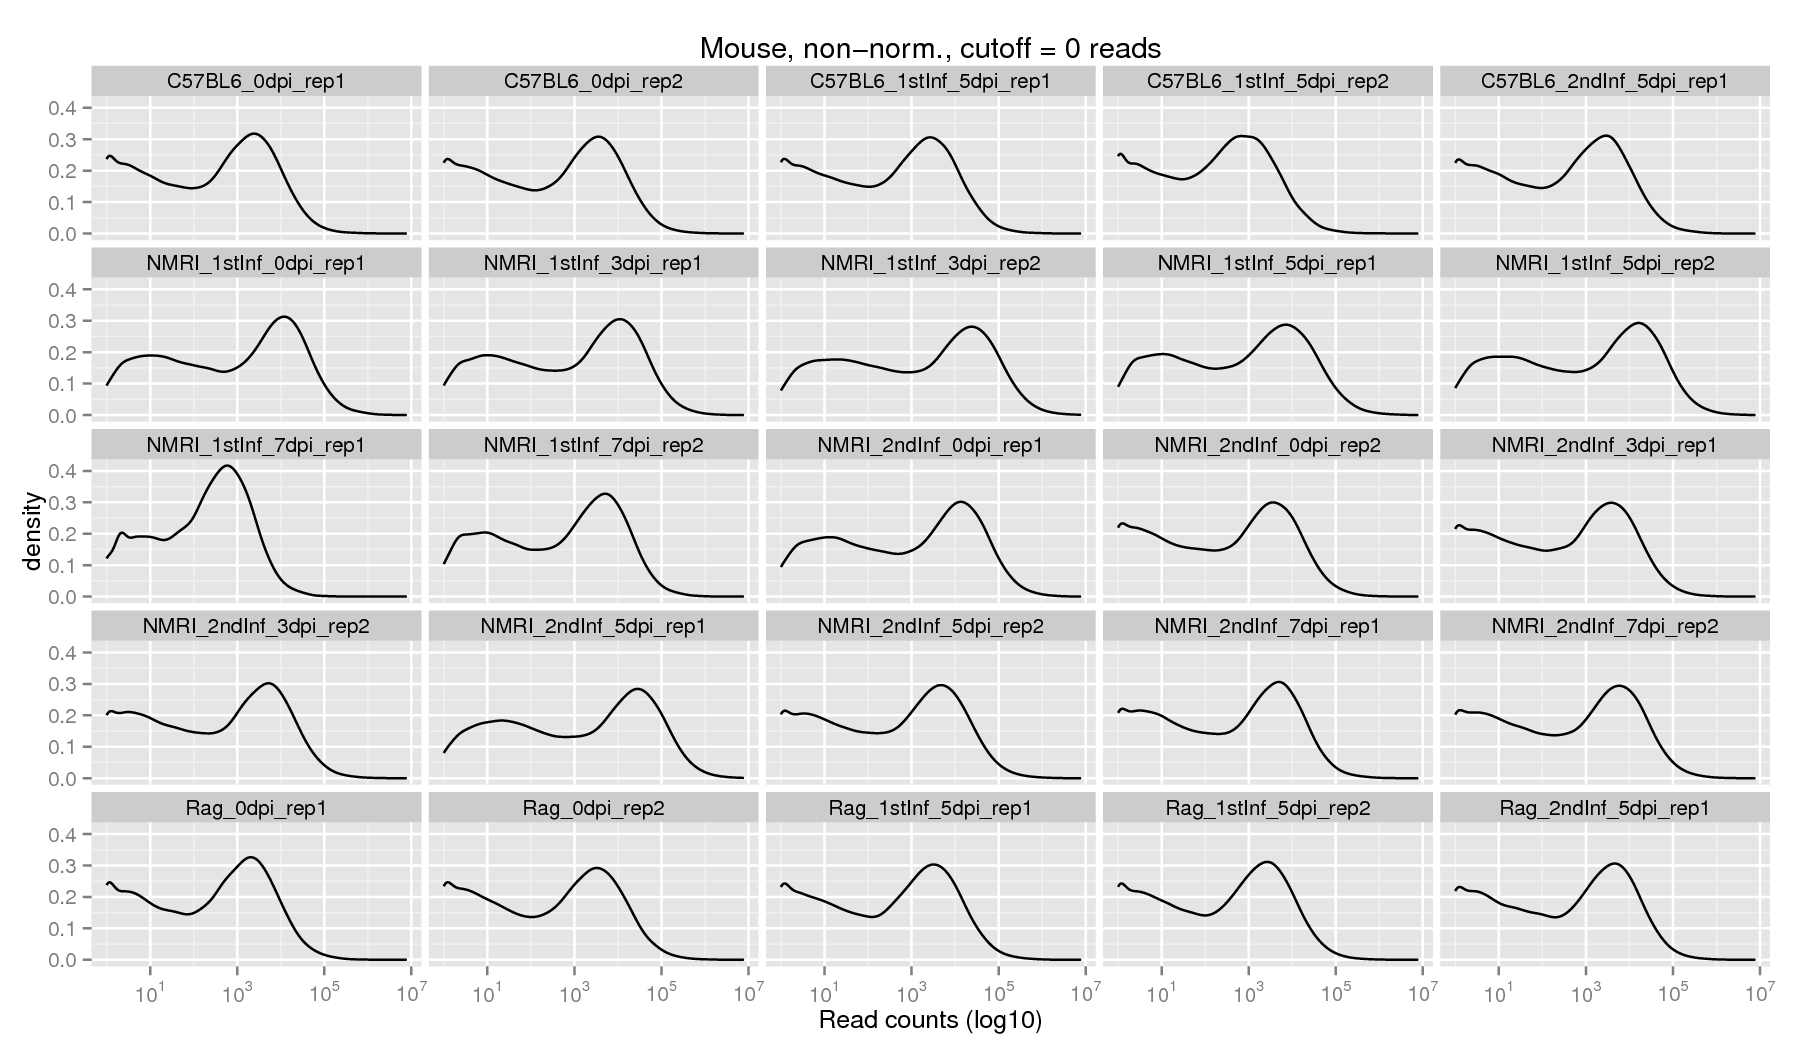
\includegraphics[width=0.8\textwidth]{distributions_mouseNocutoff} % Include the image placeholder.png
%\caption{Density distribution of raw transcript counts (log10) for all
%  mouse samples in analysis. All samples share the same bimodal
%  distribution trend by visual inspection. The first density peak
%  occur at $1 - 10^2$ transcripts, \textit{i.e.} transcripts which are
%  detected between 1 and 100 times in that sample. The second density
%  peak occurs in the range of $10^3 - 10^4$.}
%\end{center}
%\end{figure}

%----------------------------------------------------------------------------------------
%	SECTION 5
%----------------------------------------------------------------------------------------

\section{Conclusions}

Mouse\\

Parasite\\


%----------------------------------------------------------------------------------------
%	SECTION 6
%----------------------------------------------------------------------------------------

%\section{Answers to Definitions}

%\begin{enumerate}
%\begin{item}
%  The \emph{atomic weight of an element} is the relative weight of
%  one of its atoms compared to C-12 with a weight of
%  12.0000000$\ldots$, hydrogen with a weight of 1.008, to oxygen with
%  a weight of 16.00. Atomic weight is also the average weight of all
%  the atoms of that element as they occur in nature.
%\end{item}
%\begin{item}
%  The \emph{units of atomic weight} are two-fold, with an identical
%  numerical value. They are g/mole of atoms (or just g/mol) or
%  amu/atom.
%\end{item}
%\begin{item}
%  \emph{Percentage discrepancy} between an accepted (literature)
%  value and an experimental value is
%\begin{equation*}
%\frac{\mathrm{experimental\;result} - \mathrm{accepted\;result}}{\mathrm{accepted\;result}}
%\end{equation*}
%\end{item}
%\end{enumerate}

%----------------------------------------------------------------------------------------
%	BIBLIOGRAPHY
%----------------------------------------------------------------------------------------

%\bibliographystyle{apalike}

%\bibliography{sample}

%----------------------------------------------------------------------------------------


\end{document}
